\documentclass[a4paper,12pt]{article}
\usepackage{HomeWorkTemplate}
\usepackage{circuitikz}
\usepackage[shortlabels]{enumitem}
\usepackage{hyperref}
\usepackage{tikz}
\usepackage{amsmath}
\usepackage{amssymb}
\usepackage{tcolorbox}
\usepackage{xepersian}
\usepackage{graphicx}
\usepackage{tikz}
\settextfont{XB Niloofar}
\usetikzlibrary{arrows,automata}
\usetikzlibrary{circuits.logic.US}
\usepackage{changepage}
\newcounter{problemcounter}
\setcounter{problemcounter}{1}
\newcommand{\problem}[1]
{
	\subsection*{
		بخش
		\arabic{problemcounter} 
		\stepcounter{problemcounter}
		#1
	}
}


\begin{document}
\handout
{سیستم های مخابراتی}
{دکتر پاکروان}
{نیم‌سال اول 1399\lr{-}1400}
{اطلاعیه}
{صدرا صبوری هلستانی}
{97101972}
 {توضیحات پروژه درس}
\section{مقدمه}
بخش های مختلف این سیستم در دایرکتوری $./Functions$ آمده است. همچنین در همین دایرکتوری فایلی با نام $overall\_test.m$ آمده است که با اجرا آن می توان کارکرد تمامی بلوک ها را امتحان کرد.
\\
در ابتدای کار تمام توابع به گونه ای طراحی شده بودند که هم برای ورودی سطری و هم ستونی پاسخگویی داشته باشند اما سپس این پشتیبانی بعضا بسیار پر هزینه بود و بی خیال آن شدم.
\\
سعی شده است که تا جای ممکن (برای افزایش سرعت سیستم) از حلقه استفاده نشود و با برداری کردن محاسبات، سیستم را سریع تر بکنم.
\\
\\
\section{پیاده سازی بلوک ها به صورت مجزا}
\subsection{Divide and Combine}
کد تابع $Divide$ در $./Functions/Divide.m$ آمده است و در آن با گرفتن بردار ورودی، خانه های با اندیس زوج را از خانه های با اندیس فرد جدا می کنیم و به خروجی می فرستیم، مزیت این روش به نسب روش های دیگر (مثلا نصف کردن بردار ورودی از وسط) این است که اگر فرض کنیم که این سیستم می خواست به صورت واقعی عمل کند، این موضوع امکان پذیر بود (در حالت واقعی نمی توان صبر کرد تا تمام بیت ها وارد شوند و سپس آن ها را نصف کنیم، بلکه یکی در میان فرستادن آن ها انتخاب بهتری است).
\\
تابع $Combine$ نیز در $Functions/Combine\_.m$ آمده است، نام این تابع متفاوت با نام خواسته شده است، زیرا تابعی با نام مشابه جزو توابع مورد استفاده متلب است. عملکرد این تابع نیز دقیقا برعکس تابع $Divide$ است، یعنی دو دنباله ورودی را طوری کنار هم قرار می دهد که یکی در خانه های اندیس زوچ و دیگری در خانه های اندیس فرد قرار بگیرد.
\\
\subsection{PulseShaping}
کد تابع $PulseShaping$ در $./Functions/PulseShaping.m$ آمده است و در آن با گرفتن بردار ورودی، و شکل موج مرتبط با هر کدام از بیت ها با به جای هر بیت، پالس متناظر آن را جای گذاری میکند، فرکانس نمونه برداری در شکل موج های ورودی و اندازه های آن ها در نظر گرفته شده است و نیازی به آن در این مرحله نداریم.
\\
\subsection{AnalogMod}
کد تابع $AnalogMod$ در $./Functions/AnalogMod.m$ آمده است و در آن با گرفتن پالس ورودی و ساختن یک بازه زمانی به گام به اندازه زمان نمونه برداری و به اندازه طول پالس توابع سینوس و کسینوس با فرکانس حامل را روی دو سیگنال ورودی اعمال می کنیم و سپس جمع شده آن ها را به عنوان  سیگنال مدوله شده به خروجی می دهیم.
\\
\subsection{Channel}
کد تابع $Channel$ در $./Functions/Channel.m$ آمده است و در آن با گرفتن بردار ورودی تبدیل فوریه سیگنال را می گیریم و فیلتر میان گذر (با فرکانس میانی و پهنای باند داده شده) را اعمال می کنیم (چون خروجی تبدیل فوریه به صورت متقارن است، فیلتر را نیز به همین شکل روی تبدیل فوریه سیگنال اعمال می کنیم) سپس از سیگتال بدست آمده در حوزه فرکانس تبدیل عکس فوریه می گیریم و سپس از خروجی این تبدیل فوریه معکوس قسمت حقیقی آن را جدا می کنیم و آن را به عنوان خروجی کانال به خروجی ارسال می کنیم.
\\
از آن جایی که اعمال فیلتر به این شکل، فیلتر در حوزه زمان را غیر علی و غیر قابل ساخت میکند بهتر است به عنوان جایگزین یک فیلتر معمول با کمک $fdesign$ طراحی کنیم و این فیلتر را در حوزه فرکانس در تبدیل فوریه سیگنال ضرب کنیم و سپس مانند حالت فعلی عمل کنیم، مشخصا نتیجه کمی ضعیف تر خواهد بود ولی در عوض به نتیجه فیزیکی در دنیای واقعی نزدیک خواهیم شد.
\\
\subsection{AnalogDemod}
کد تابع $AnalogDemod$ در $./Functions/AnalogDemod.m$ آمده است و در آن گونه ای کار های مشابه دو تابع قبل را انجام می دهیم، ابتدا سیگنال ورودی را یکبار در سینوس و یکبار در کسینوس با فرکانس حامل داده شده ضرب می کنیم و دو سیگنال خروجی را از فیلتر های پایین گذر (فرآیند مشابه تابع $Channel$ اعمال می کنیم) و این دو سیگنال را به خروجی می بریم.
\\
\subsection{MatchFilt}
کد تابع $MatchedFilt$ در $./Functions/MatchedFilt.m$ آمده است، در این تابع با توجه به اینکه بهترین تابع به عنوان پاسخ ضربه سیستم خود شکل پالس ها هستند که در بازه زمان برعکس شده اند و به اندازه $T$ جا به جا شده است و برای بدست آوردن خروجی این فیلتر باید به گونه ای سیگنال را با قرینه زمانی یک سیگنال کانولوشن کنیم که این کار معادل کورلیشن است.
\\
\subparagraph{آ)}
برای این کار سیگنال ورودی را به اندازه پالس ها جدا میکنیم (برای سریع تر شدن ماتریس را از حالت تک بعدی به چند بعدی تغییر می دهیم و محاسبات را به صورت ماتریسی روی سطر ها انجام می دهیم)، سپس یکبار کورلیشن این ماتریس (هر سطر به صورت جداگانه) را با هر کدام از شکل موج های متناظر با 0 و 1 انجام می دهیم و خانه وسط (نقطه متناظر با T) آن را به عنوان حاصل نهایی کورلیشن انتخاب میکنیم در نتیجه برای هر نمونه یک عدد داریم، این 2 بردار را به عنوان خروجی $MatchedFilter$ برمی گردانیم
\\
\subparagraph{ب)}
دو بردار بدست آمده از قسمت قبل را به ازای هر خانه با یک دیگر مقایسه میکنیم و جایی که بردار مربوط به کورلیشن سیگنال با پالس 1 بیشتر است نمونه متناظر را برابر با بیت 1 در نظر می گیریم و در غیر این آن را صفر میکنیم (برای حالت مساوی هم صفر در نظر گرفته شده است، اما به صورت معمول - با پالس های با معنی و متفاوت برای 0 و 1 - این حالت بسیار نادر است).
\\
\clearpage
\section{انتقال دنباله ی تصادفی صفر و یک}
کد های مربوط به این قسمت را می توانید در $./3.Transferring0and1/$ مشاهده کنید.
\subsection{0,1 PulseShaping}
مطابق خواسته ی سوال با توجه به طول پالس و فرکانس نمونه برداری یک بردار $T_p \times f_s = 10ms \times 1MHz = 10000 $ تایی یکبار همه 1 و بار دیگر همه -1 تولید می کنیم تا به عنوان پالس های متناظر با 1 و 0 آن ها را به سیستم معرفی بکنیم.
\\
ضمنا کد های مروبط به این قسمت را میتوانید در همان دایرکتوری با نام های به شکل $Q1P*.m$ مشاهد کنید.
\subparagraph{آ)}
خروجی سیستم در هر کدام از حالت ها را در شکل زیر آمده اند، این کار را در حالت عدم وجود نویز به تعداد متفاوت دنباله ورودی به شکل زیر می بینیم:
\begin{figure}[htbp]
\centerline{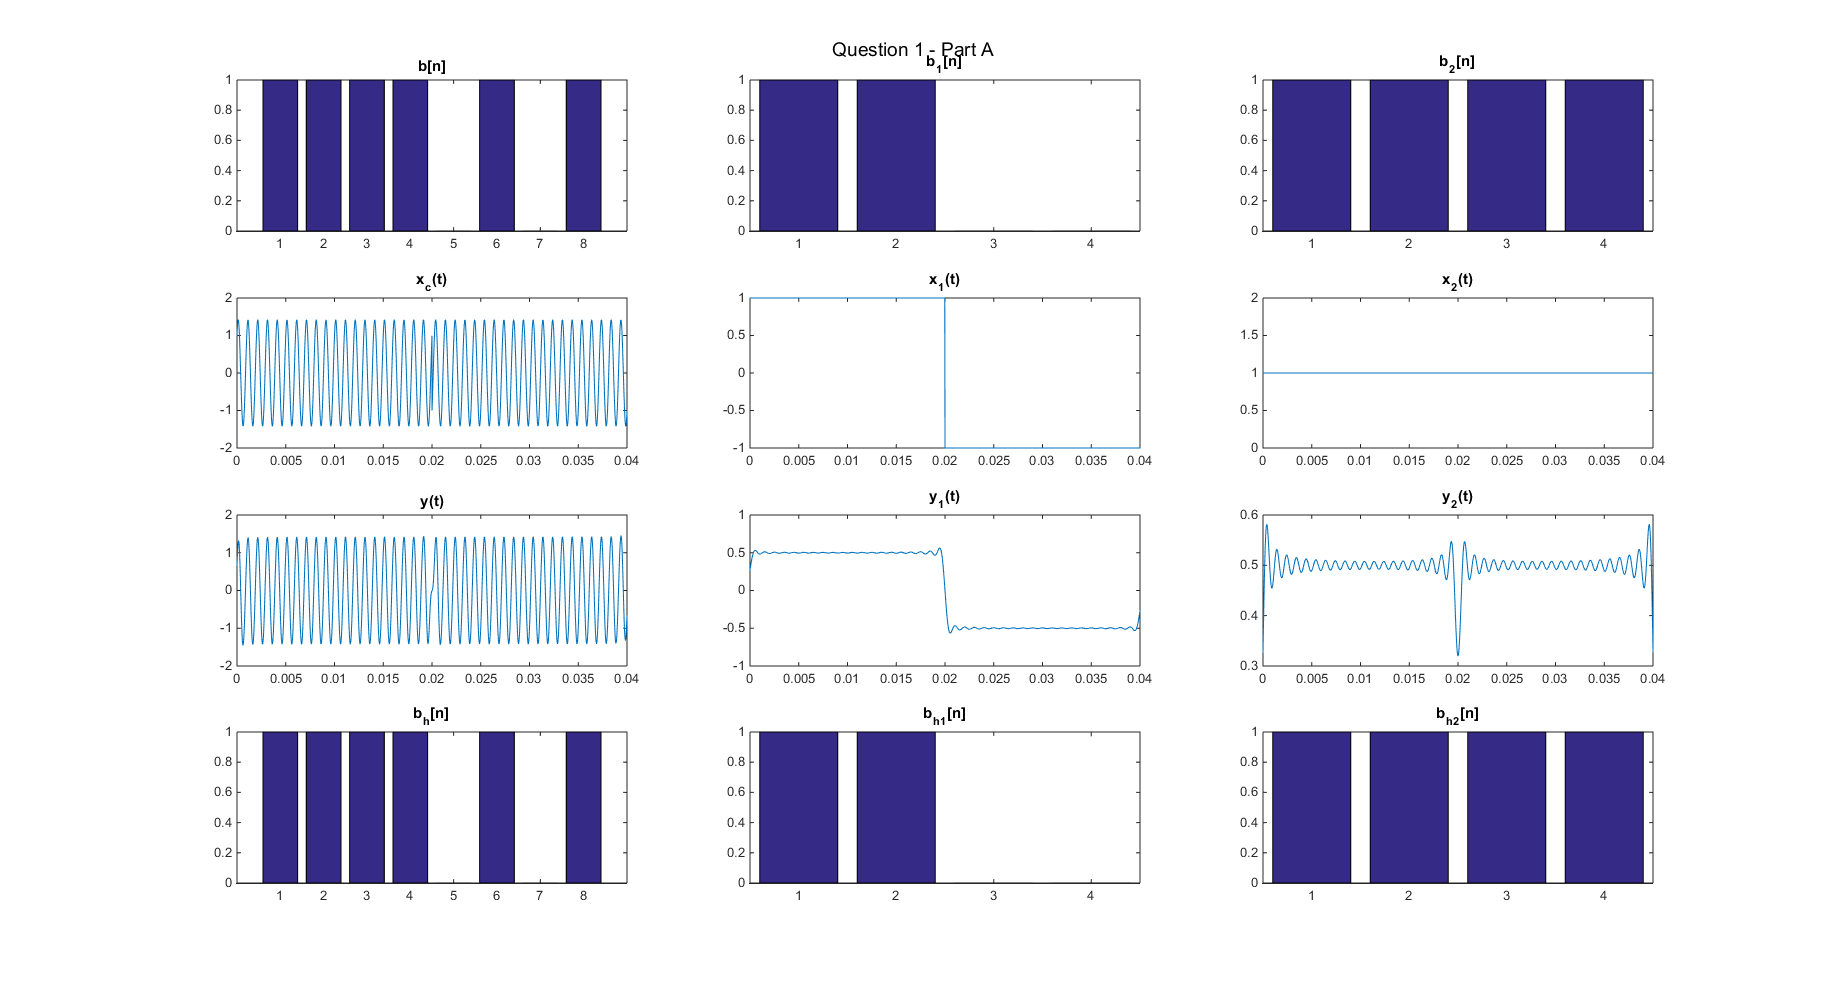
\includegraphics[width=6.625in, height=4in]{../3.Transferring0and1/Q1PA_8.png}}
\caption{خروجی قسمت های مختلف در عدم حضور نویز و با طول دنباله 8 بیت}
\label{fig}
\end{figure}
\begin{figure}[htbp]
\centerline{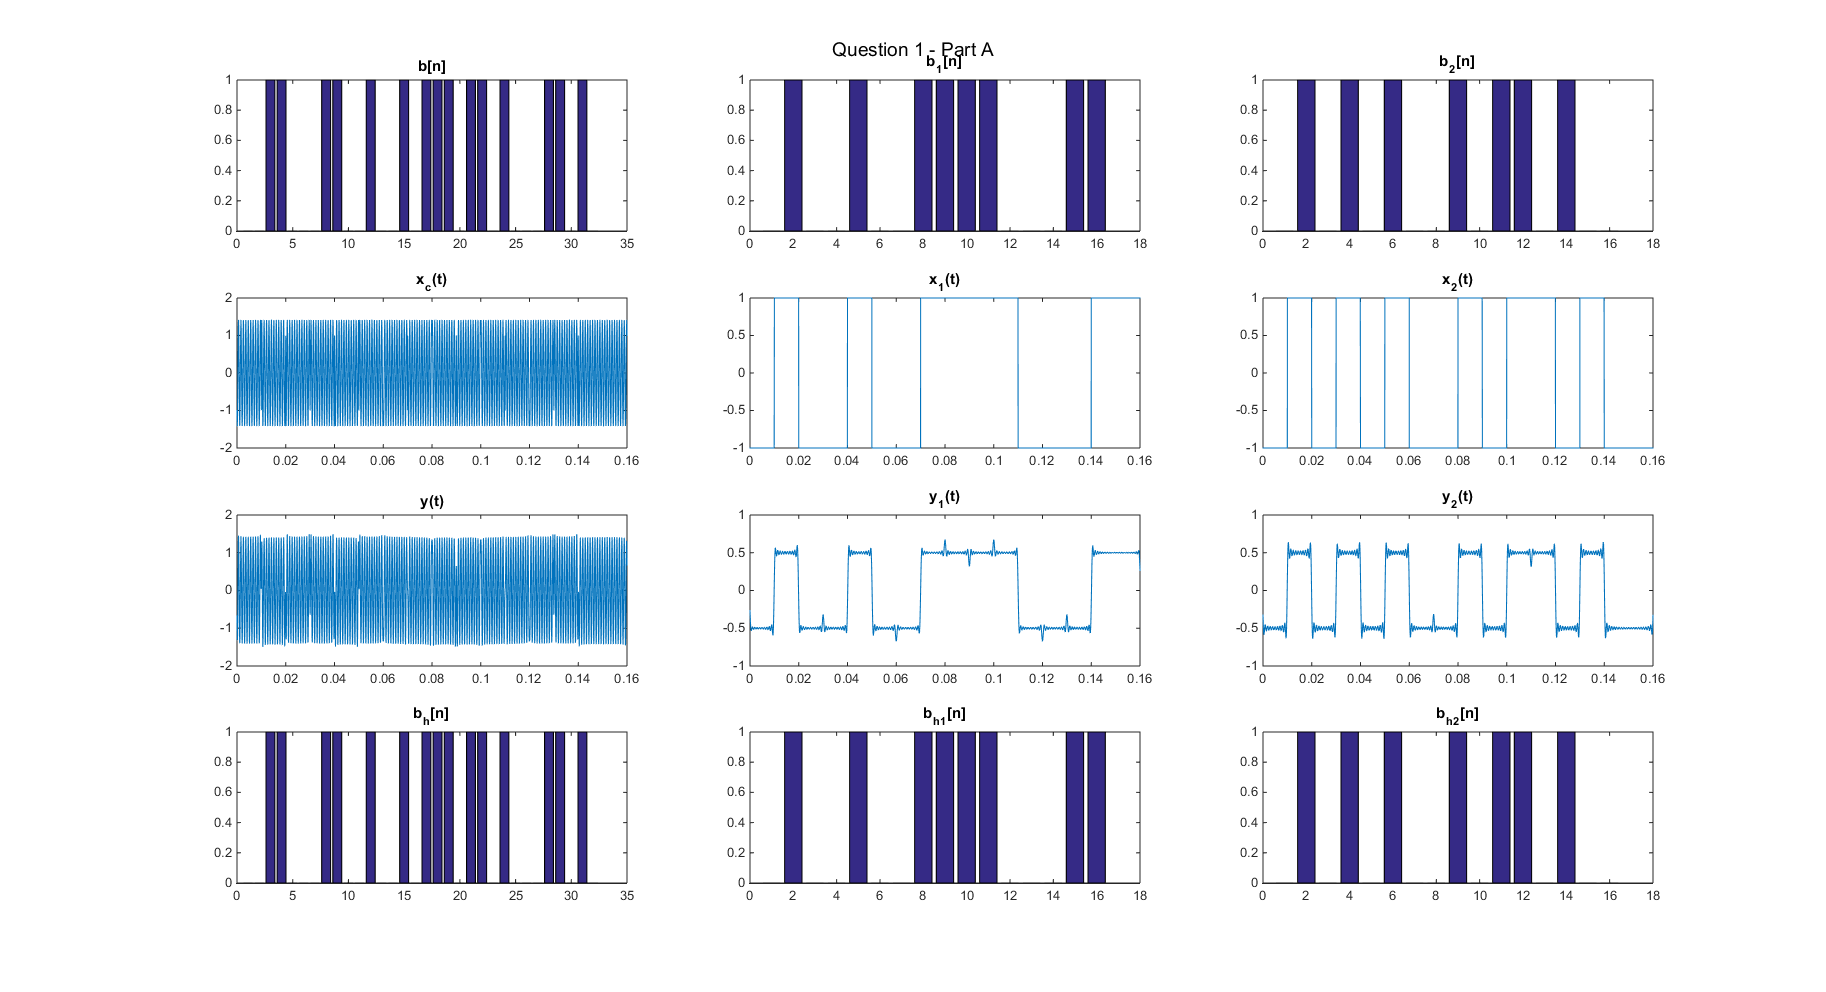
\includegraphics[width=6.625in, height=4in]{../3.Transferring0and1/Q1PA_32.png}}
\caption{خروجی قسمت های مختلف در عدم حضور نویز و با طول دنباله 32 بیت}
\label{fig}
\end{figure}
\begin{figure}[htbp]
\centerline{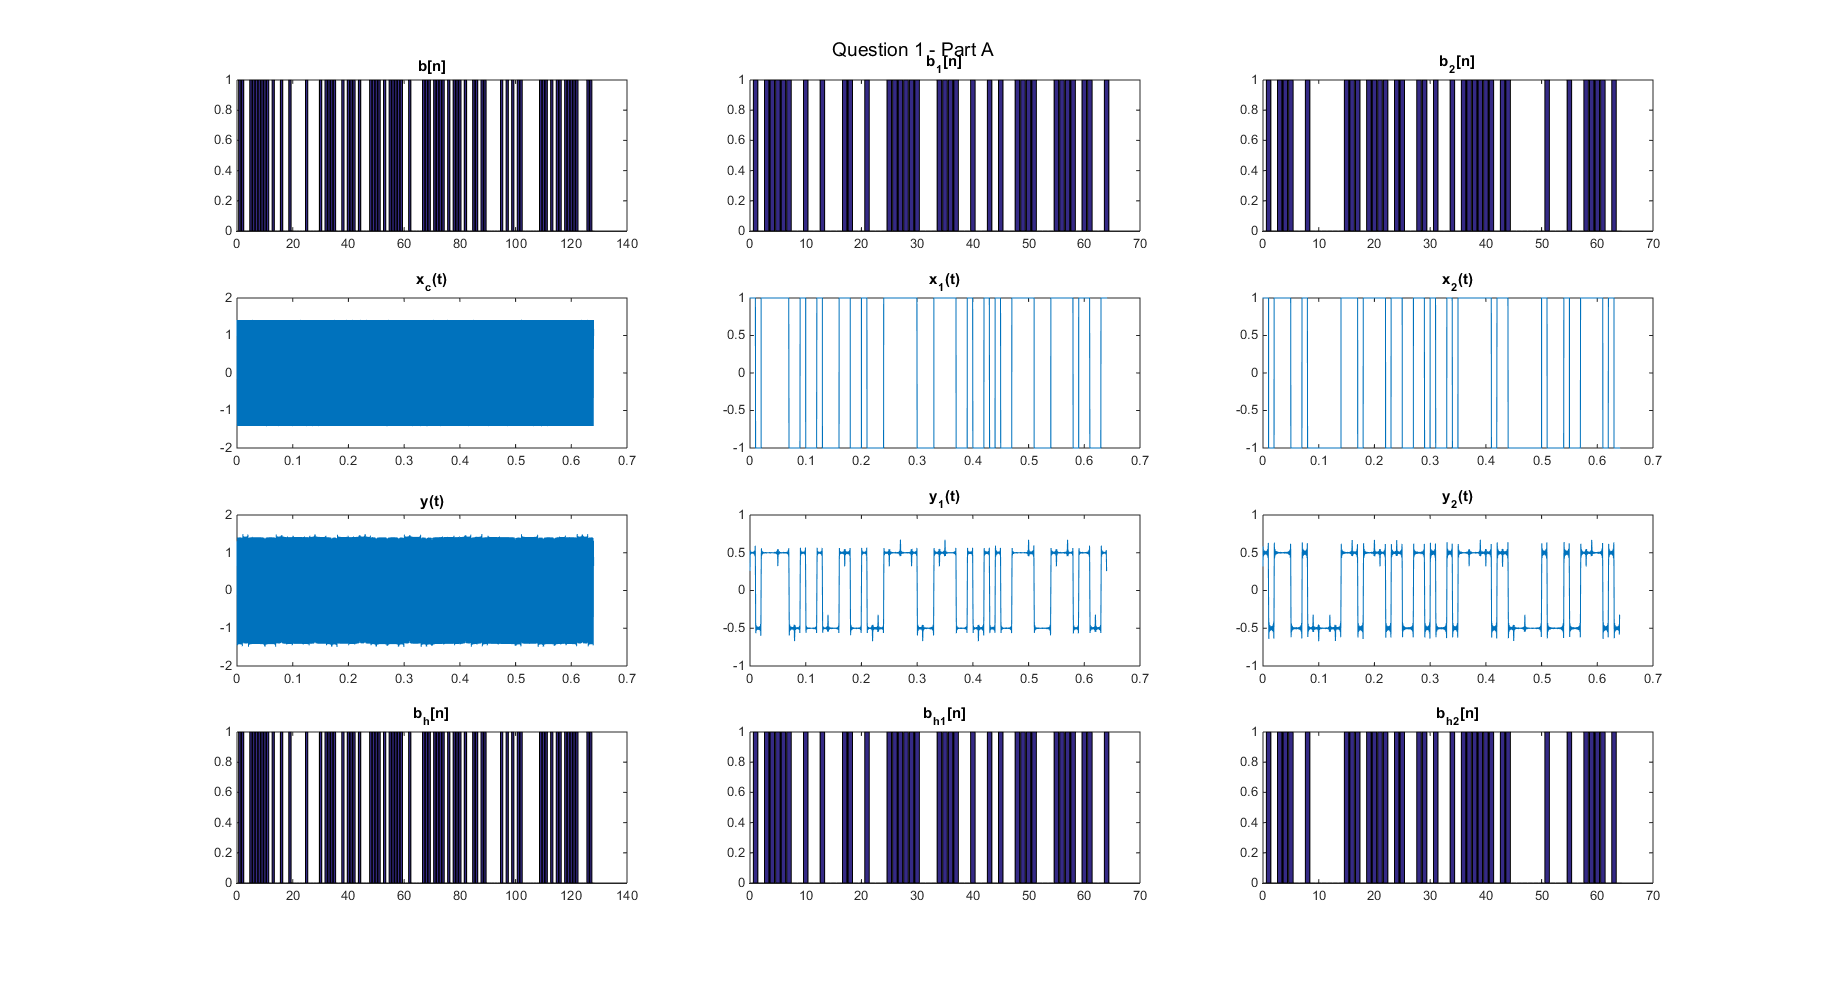
\includegraphics[width=6.625in, height=4in]{../3.Transferring0and1/Q1PA_128.png}}
\caption{خروجی قسمت های مختلف در عدم حضور نویز و با طول دنباله 128 بیت}
\label{fig}
\end{figure}
برای نمایش بیت ها از تابع $bar$ استفاده شده است که خروجی را مانند بارکد نشان میدهد، جا هایی که رنگی است یعنی بیت 1 است و جاهایی که سفید است یعنی 0 است.
\\
مشهود ترین نکته در این نمودار ها تاثیر کانال روی سیگنال ها هست که به دلیل حذف شدن فرکانس های بالاتر آن ها کمی فرم مربعی خود را از دست داده اند.
\clearpage
\subparagraph{ب)}
برای اضافه کردن نویز سفید گوسی از تابع $awgn$ متلب استفاده کردیم که با گرفتن سیگنال و $SNR$ مورد نظر (بر حسب $dB$) نویز مناسب را به سیگنال اضافه می کند و در خروجی تحویل می دهد، ضمنا از رابطه زیر با فرض 1 بودن توان سیگنال استفاده کردیم:
$$
SNR(dB) = log_{10}(\frac{\frac{N_0}{2}}{\sigma_n^2})
$$
برای این قسمت کافی است از کد قبلی استفاده بکنیم ولی این بار در یک حلقه به خروجی کانال نویز های مختلف را اضافه کنیم و تعداد بیت های اشتباه شده را ($0$ بوده و $1$ شدند یا برعکس) با $XOR$ کردن دنباله ورودی با دنباله بدست آمده  و میانگین گیری از این خطا، میزان خطا بدست می آید، بدیهتا بیشترین خطا زمانی رخ می دهد که ورودی و خروجی کاملا از هم مستقل باشند و در آن صورت میزان این خطا برابر $0.5$ است.
\\
برای این حالت نیز به ازای 2 اندازه دنباله بیت نمودار خطای تجربی بدست آمده بر حسب واریانس نویز به شکل های زیر می باشد:
\begin{figure}[htbp]
\centerline{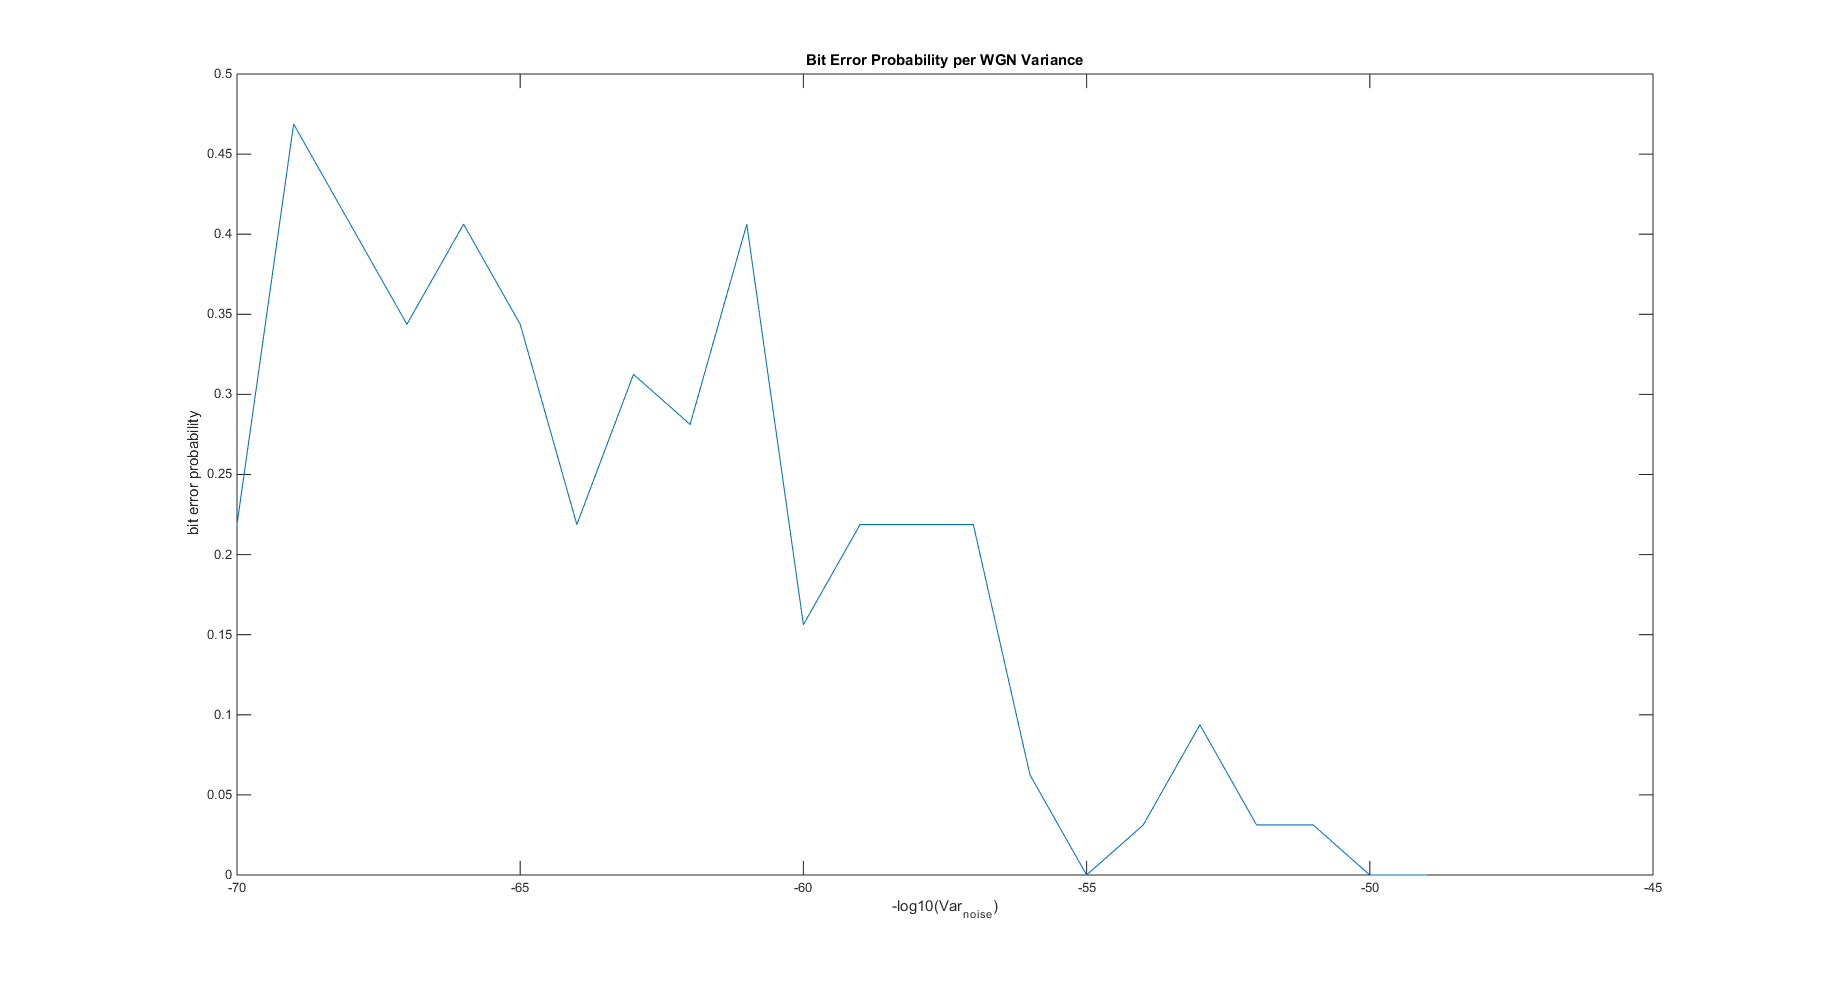
\includegraphics[width=3.125in, height=2in]{../3.Transferring0and1/Q1PB_32.png}}
\caption{نمودار خطای بیت بر حسب واریانس نویز با طول دنباله 8 بیت}
\label{fig}
\end{figure}
\begin{figure}[htbp]
\centerline{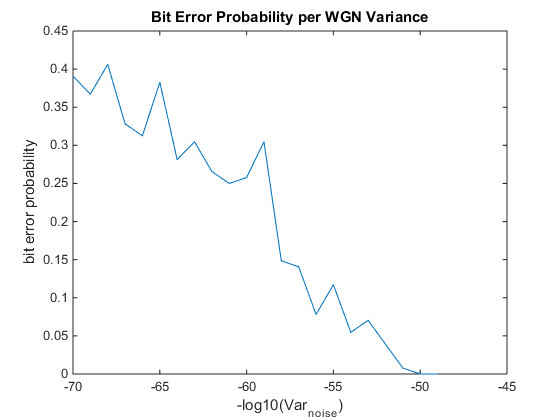
\includegraphics[width=3.125in, height=2in]{../3.Transferring0and1/Q1PB_128.png}}
\caption{نمودار خطای بیت بر حسب واریانس نویز با طول دنباله 128 بیت}
\label{fig}
\end{figure}
همانطور که دیده می شود از واریانس $10^{50}$ نویز خطا کم کم شروع می شود و در مقدار $10^{70}$ به مقدار ماکسیموم خود یعنی $0.5$ می رسد.
\clearpage
\subparagraph{ج)}
برای این کار با توجه به نمودار های قسمت قبل 6 واریانس متفاوت را انتخاب می کنیم به قسمی  که تمام بازه را پوشش می دهد، این توان ها عبارت اند از:
$$
\sigma^2 = \{10^{100}, 10^{80}, 10^{60}, 10^{40}, 10^{20}, 1\}
$$
و نیز با توجه به توضیحات آقای رحمانی در کلاس توجیهی پروژه از آن جایی که از آن جایی که میخواهیم این نمودار را روی بازه $(-1,-1)$ نشان دهیم می بایست مقادیر خروجی $MatchFilter$ که در آن ها صفر تشخیص داده شده اند، را در منفی ضرب کنیم تا به این شکل به کمک خروجی های فیلتر برای دو دنباله نصف شده $\hat{b_1}$ و $\hat{b_2}$ اولی به عنوان مختص محور $x$ و دومی به عنوان مختص محور $y$ مورد استفاده میگیرد.
\\
ضمنا در حال محاسبه هر کدام از آن ها قسمت مربوطه به آنان در نمودا تکمیل میگیرد و به کمک $scatter$ روی فضای 2 بعدی نشان داده شده اند، برای درک بهتر تصمیم گرفته شده است که خطوط محور ها هم رسم شوند تا مرز جدایی آنان بیشتر مشخص شود.
\begin{figure}[htbp]
\centerline{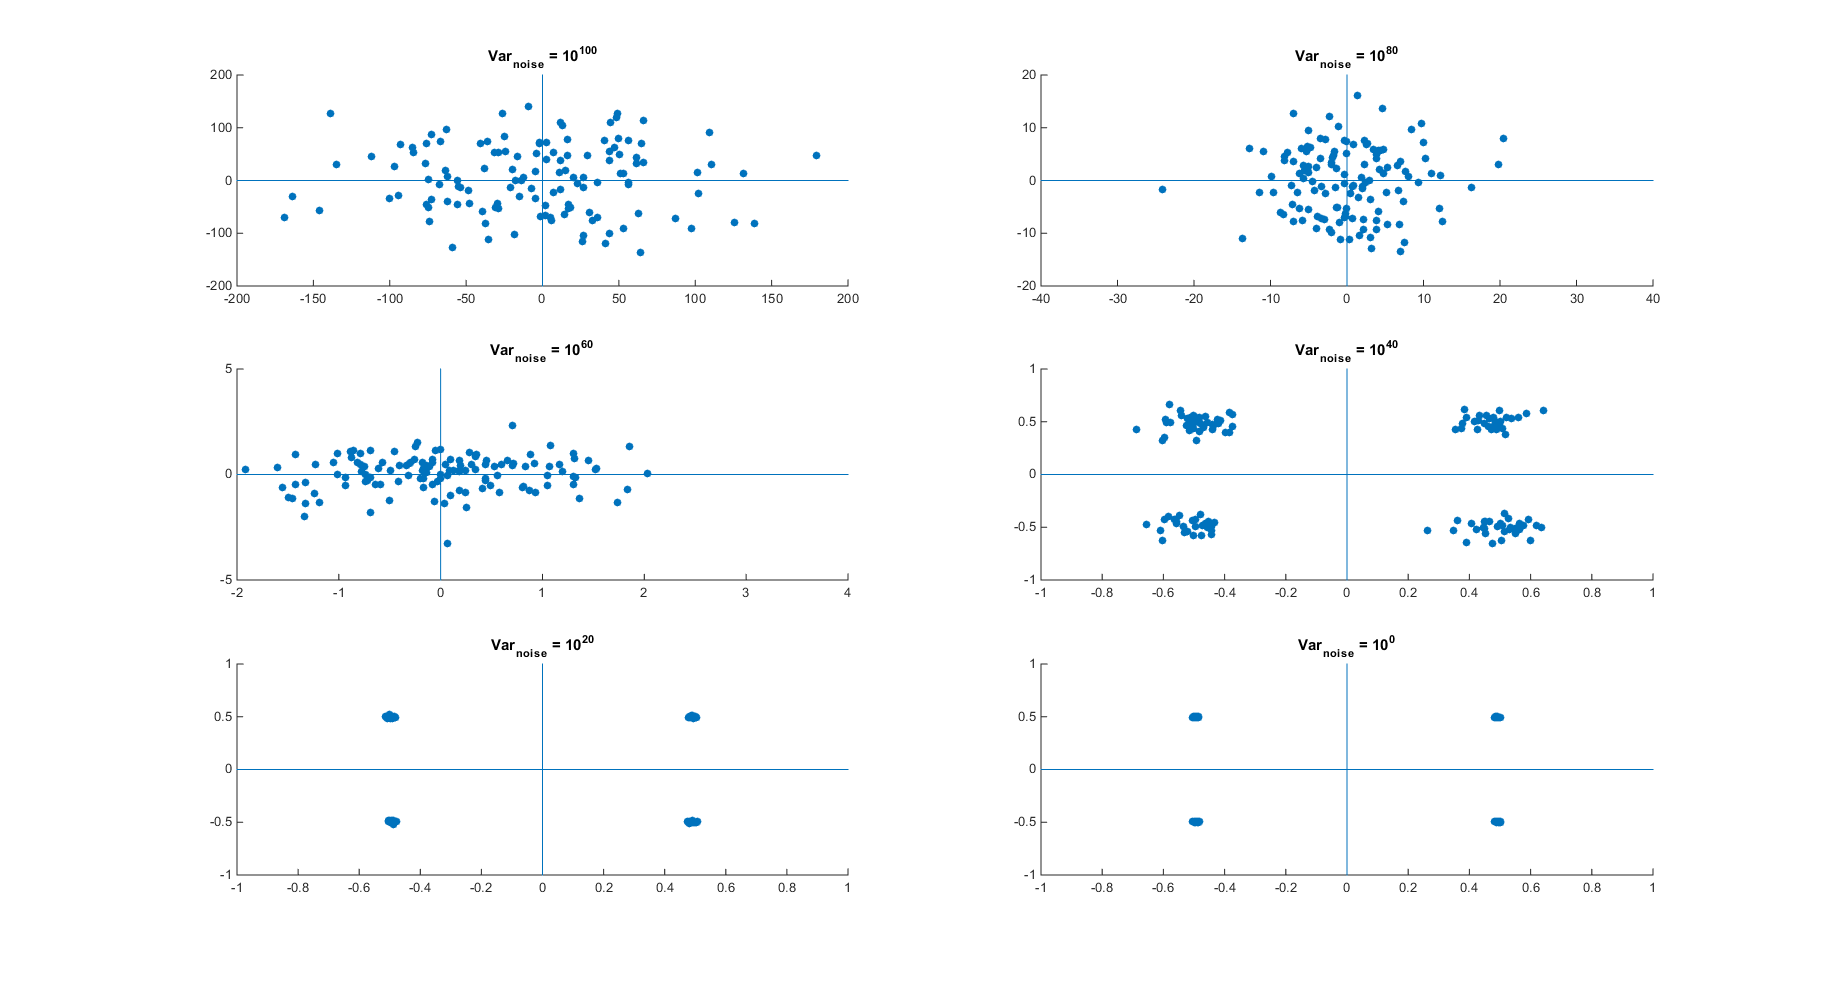
\includegraphics[width=6.625in, height=4in]{../3.Transferring0and1/Q1PC.png}}
\caption{توزیع خطا در فضای 2 بعدی به ازای دنباله 128 بیتی}
\label{fig}
\end{figure}
همانطور که دیده می شود با افزایش واریانس نویز ابر دور نقاط صحیح پیوسته بزرگتر می شود، در توان $10^{40}$ هنوز خطا قابل قبول است اما همانطور که دیده می شود در گام بعدی ابر ها کاملا با هم قاطی شده اند و دیگر نمی توان بیت ها را به صورت درست بازیابی کرد.
\clearpage

\subsection{Sine PulseShaping}
مطابق خواسته ی سوال با توجه به طول پالس و فرکانس نمونه برداری یک بردار $T_p \times f_s = 10ms \times 1MHz = 10000 $ به عنوان بردار زمان تعریف میکنیم و سپس با استفاده از آن مقدار $sin(2\pi500t)$ و $sin(2\pi500t)-$ در این بازه بدست آوریم و به ترتیب به عنوان شکل موچ مربوط به 1 و 0 معرفی میکنیم.
\\
ضمنا کد های مروبط به این قسمت را میتوانید در همان دایرکتوری با نام های به شکل $Q2P*.m$ مشاهد کنید.
\subparagraph{آ)}
خروجی سیستم در هر کدام از حالت ها را در شکل زیر آمده اند، این کار را در حالت عدم وجود نویز به تعداد متفاوت دنباله ورودی به شکل زیر می بینیم:
\begin{figure}[htbp]
\centerline{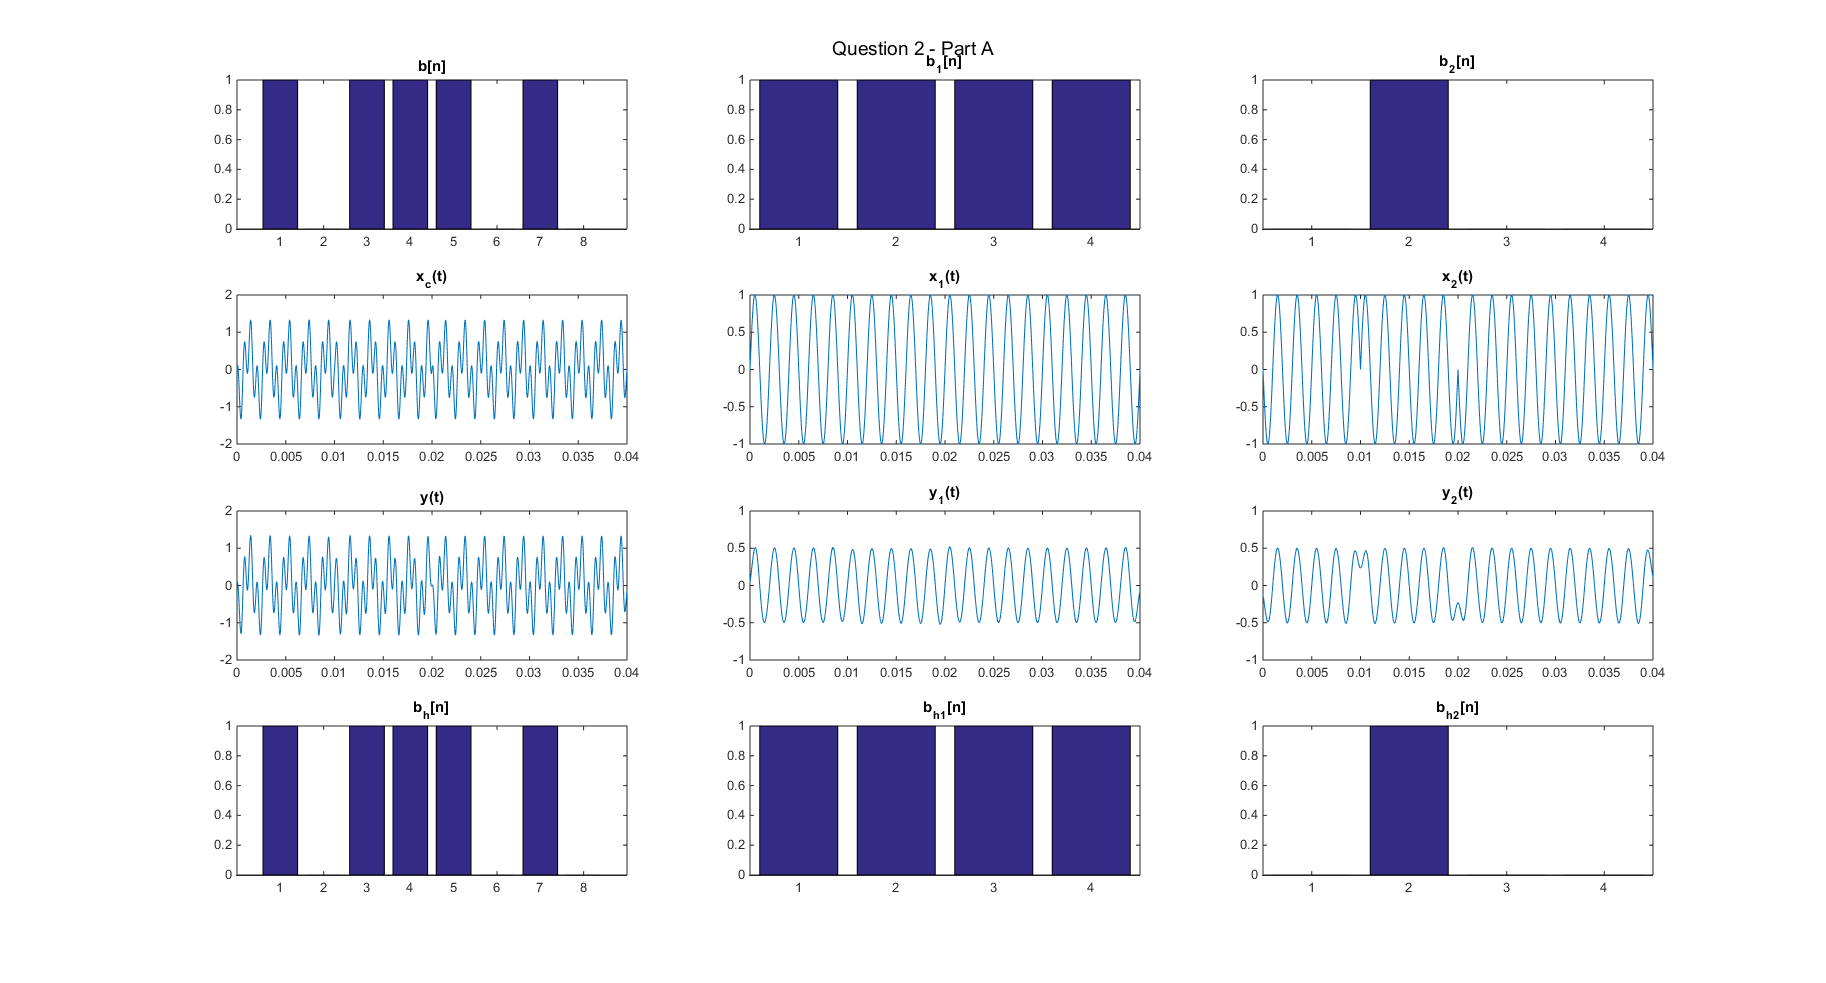
\includegraphics[width=6.625in, height=4in]{../3.Transferring0and1/Q2PA_8.png}}
\caption{خروجی قسمت های مختلف در عدم حضور نویز و با طول دنباله 8 بیت}
\label{fig}
\end{figure}
\begin{figure}[htbp]
\centerline{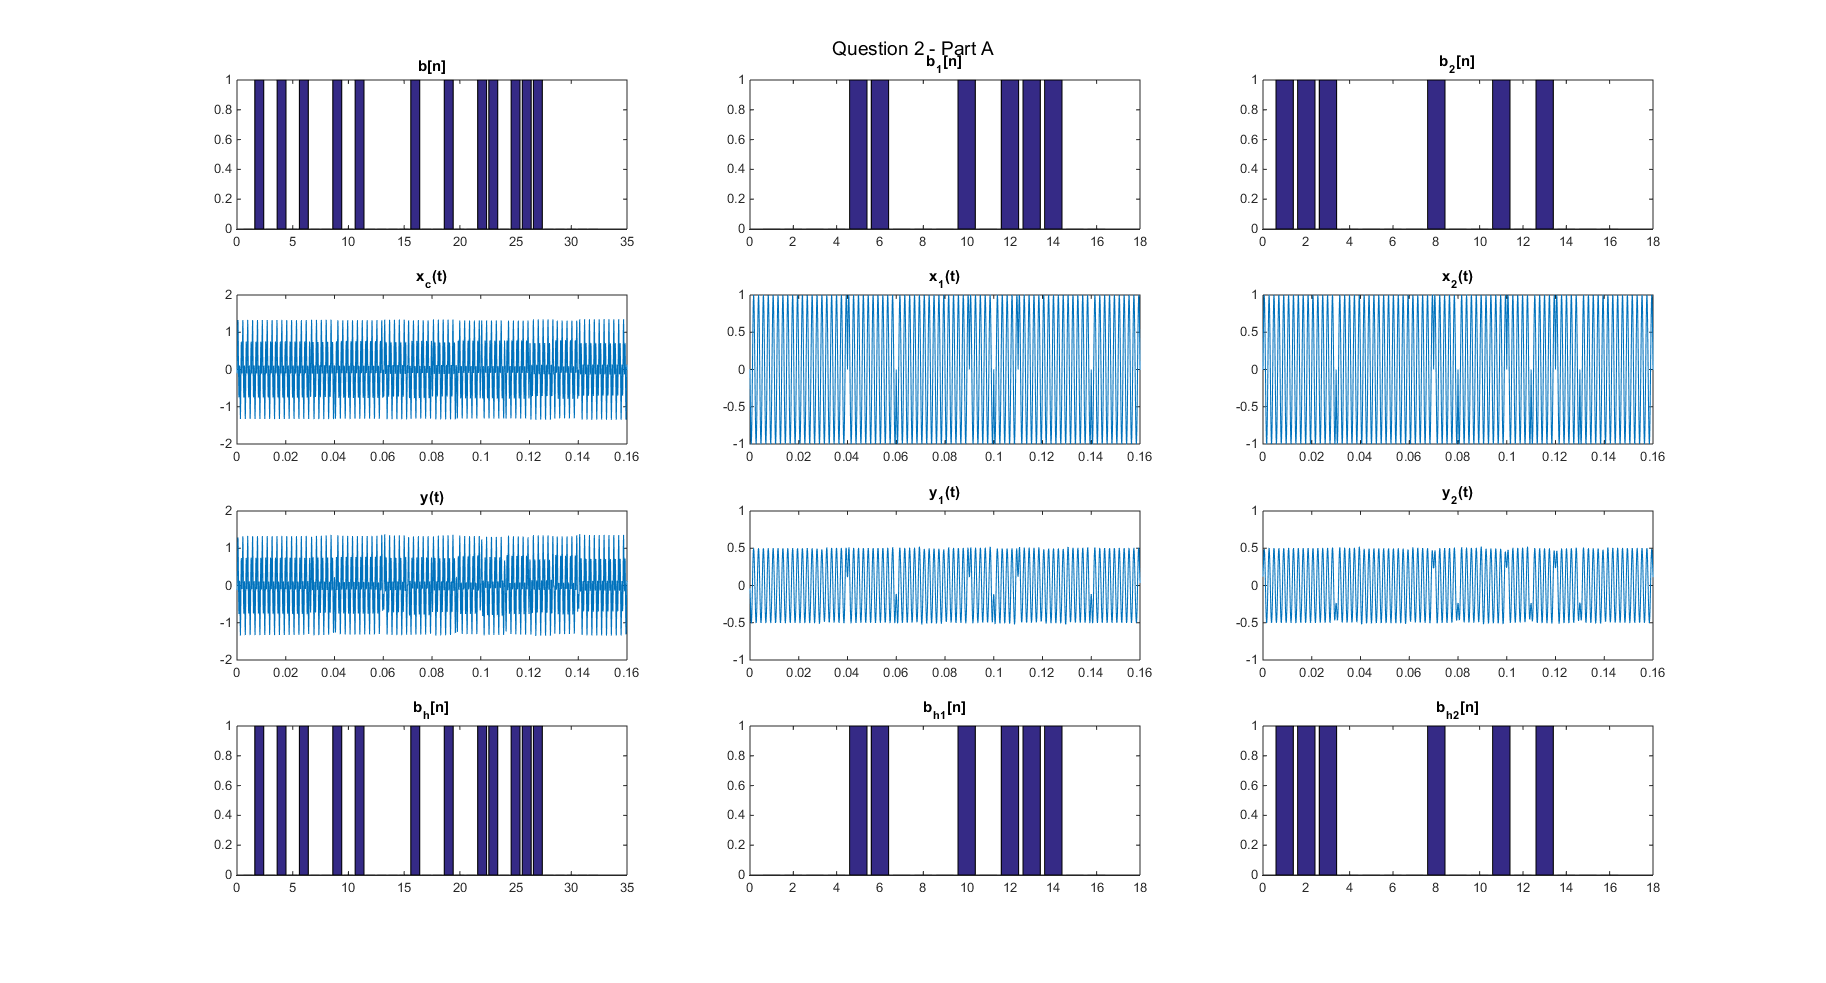
\includegraphics[width=6.625in, height=4in]{../3.Transferring0and1/Q2PA_32.png}}
\caption{خروجی قسمت های مختلف در عدم حضور نویز و با طول دنباله 32 بیت}
\label{fig}
\end{figure}
\begin{figure}[htbp]
\centerline{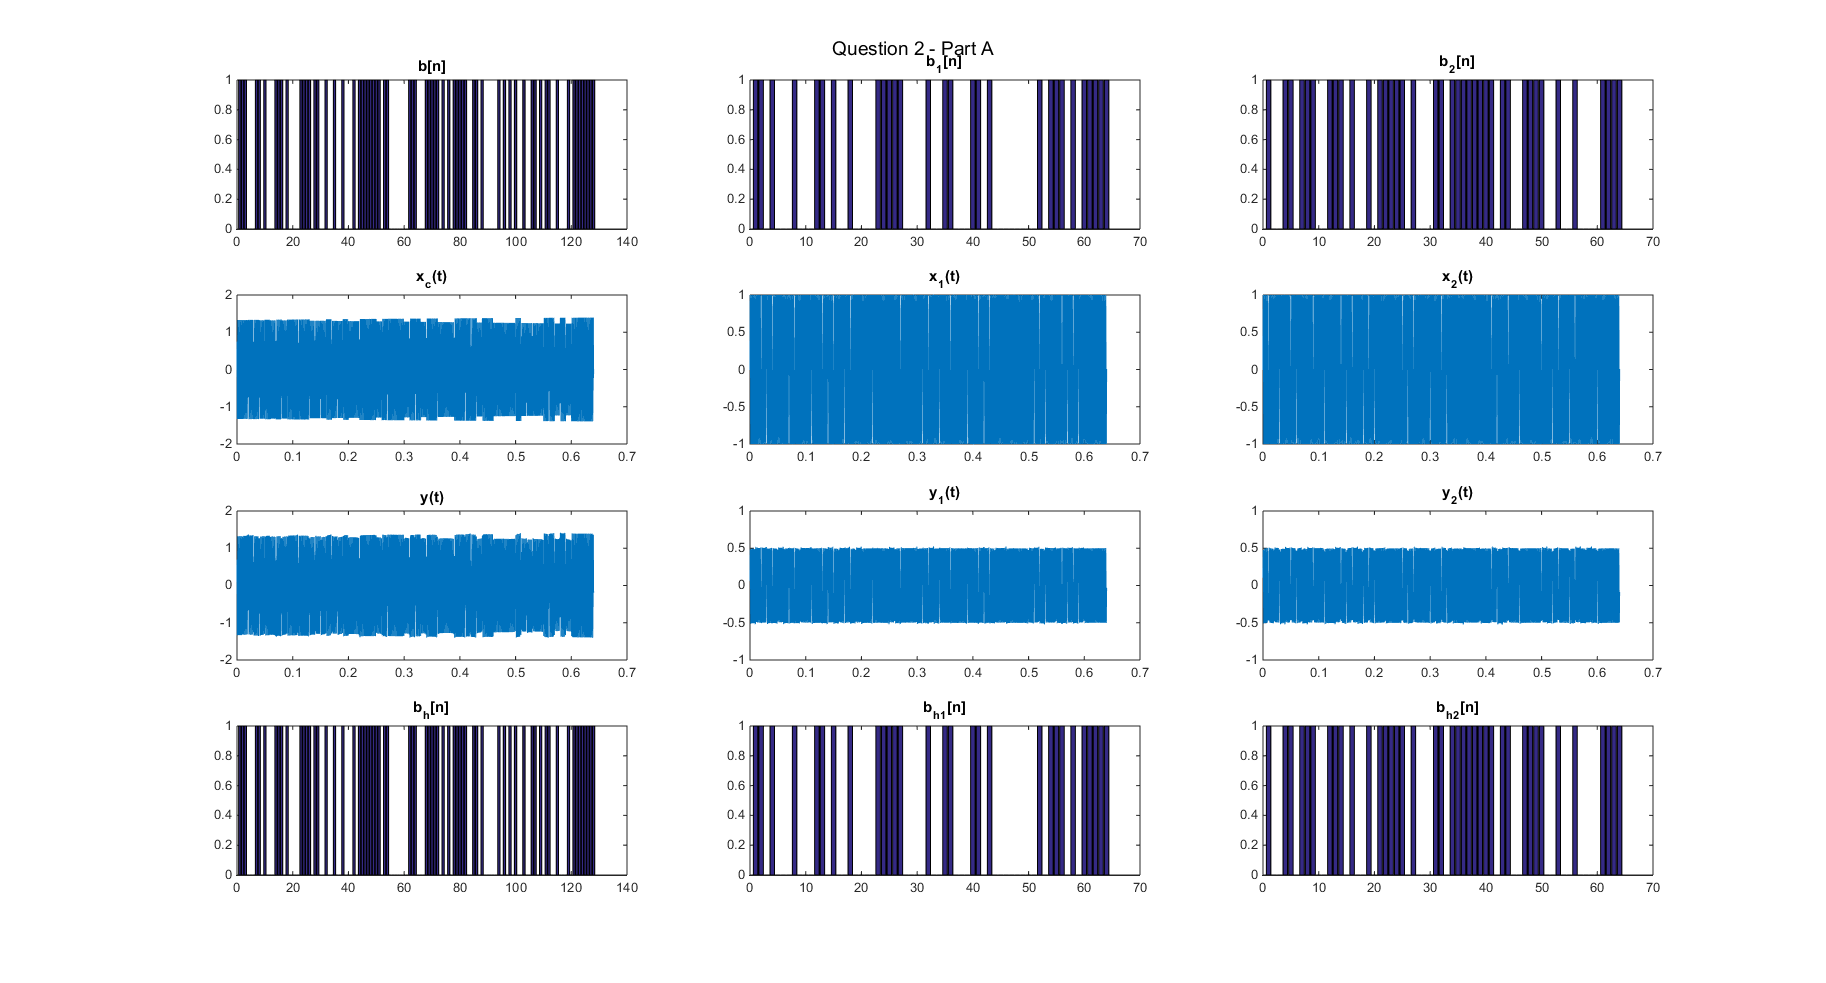
\includegraphics[width=6.625in, height=4in]{../3.Transferring0and1/Q2PA_128.png}}
\caption{خروجی قسمت های مختلف در عدم حضور نویز و با طول دنباله 128 بیت}
\label{fig}
\end{figure}
برای نمایش بیت ها از تابع $bar$ استفاده شده است که خروجی را مانند بارکد نشان میدهد، جا هایی که رنگی است یعنی بیت 1 است و جاهایی که سفید است یعنی 0 است.
\\
مشهود ترین نکته در این نمودار ها تاثیر کانال روی سیگنال ها هست که به دلیل حذف شدن فرکانس های بالاتر آن ها کمی فرم مربعی خود را از دست داده اند.
\\
تفاوت دیگری که دیده میشود این است که پالس های تولید شده در این حالت خیلی متخلخل تر و در هم تر هستند و جداسازی آنان به کمک چشم (و احتمالا به کمک $MatchFilter$ سخت تر است) و نسبت به نویز ضعف بیشتری خواهد داشت. تغییر وضعیت بیت ها را از ناحیه های سفیدی که در اثر عوض شدن مشتق تابع به صورت ناگهانی پدید آمده اند دیده می شود.
\clearpage
\subparagraph{ب)}
برای این قسمت کافی است از مشابه کد قبلی عمل بکنیم.
\\
برای این حالت نیز به ازای 2 اندازه دنباله بیت نمودار خطای تجربی بدست آمده بر حسب واریانس نویز به شکل های زیر می باشد:
\begin{figure}[htbp]
\centerline{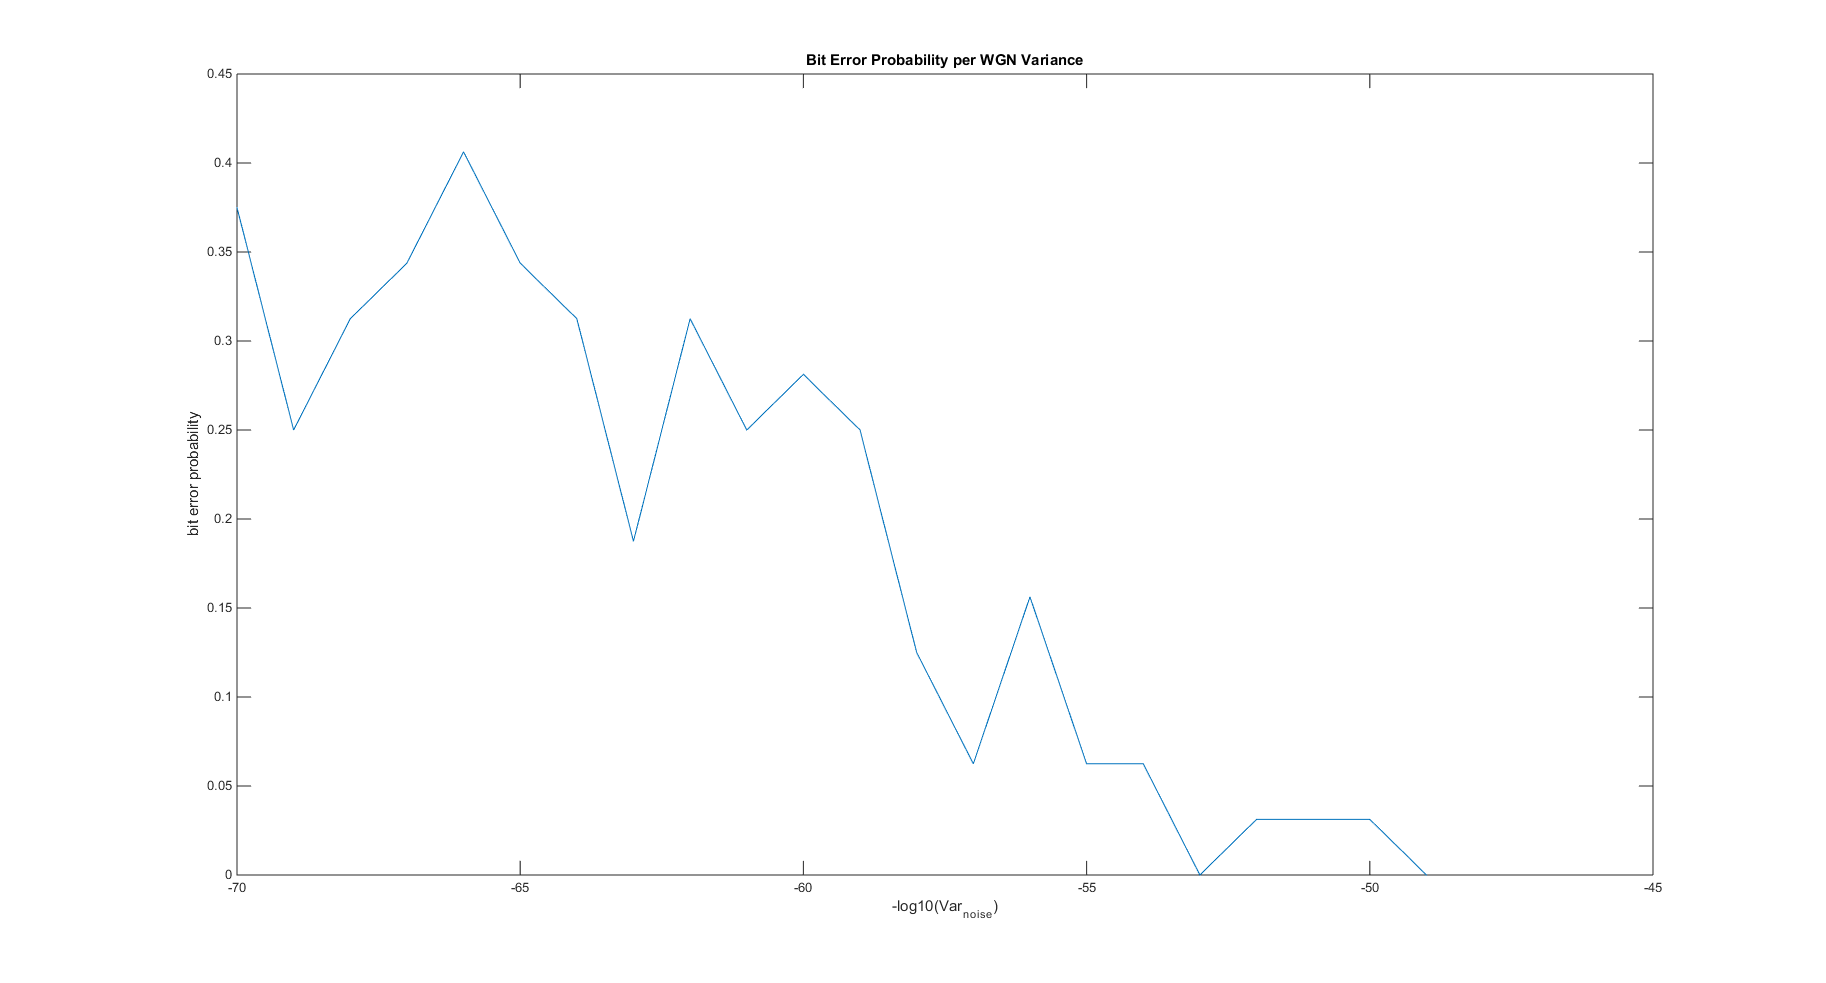
\includegraphics[width=3.125in, height=2in]{../3.Transferring0and1/Q2PB_32.png}}
\caption{نمودار خطای بیت بر حسب واریانس نویز با طول دنباله 8 بیت}
\label{fig}
\end{figure}
\begin{figure}[htbp]
\centerline{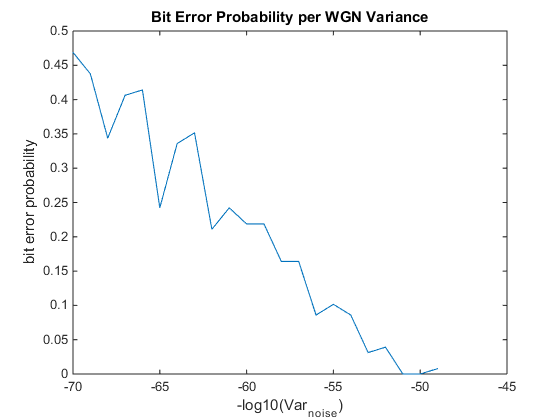
\includegraphics[width=3.125in, height=2in]{../3.Transferring0and1/Q2PB_128.png}}
\caption{نمودار خطای بیت بر حسب واریانس نویز با طول دنباله 128 بیت}
\label{fig}
\end{figure}
همانطور که دیده می شود از واریانس $10^{50}$ نویز خطا کم کم شروع می شود و در مقدار $10^{70}$ به مقدار ماکسیموم خود یعنی $0.5$ می رسد. (این نمودار آنچنان نشان دهنده تفاوت نیست، ولی در همین جا هم مشخص است که نویز در توان کوچک تری شروع به تغییر بیت ها کرده است که این نشان دهنده ضعف در مقابل نویز است)
\clearpage
\subparagraph{ج)}
برای این کار با توجه به نمودار های قسمت قبل همان 6 واریانس قسمت قبل را انتخاب می کنیم به قسمی  که تمام بازه را پوشش می دهد، این توان ها عبارت اند از:
$$
\sigma^2 = \{10^{100}, 10^{80}, 10^{60}, 10^{40}, 10^{20}, 1\}
$$
و نیز با توجه به توضیحات آقای رحمانی در کلاس توجیهی پروژه از آن جایی که از آن جایی که میخواهیم این نمودار را روی بازه $(-1,-1)$ نشان دهیم می بایست مقادیر خروجی $MatchFilter$ که در آن ها صفر تشخیص داده شده اند، را در منفی ضرب کنیم تا به این شکل به کمک خروجی های فیلتر برای دو دنباله نصف شده $\hat{b_1}$ و $\hat{b_2}$ اولی به عنوان مختص محور $x$ و دومی به عنوان مختص محور $y$ مورد استفاده میگیرد.
\\
ضمنا در حال محاسبه هر کدام از آن ها قسمت مربوطه به آنان در نمودا تکمیل میگیرد و به کمک $scatter$ روی فضای 2 بعدی نشان داده شده اند، برای درک بهتر تصمیم گرفته شده است که خطوط محور ها هم رسم شوند تا مرز جدایی آنان بیشتر مشخص شود.
\begin{figure}[htbp]
\centerline{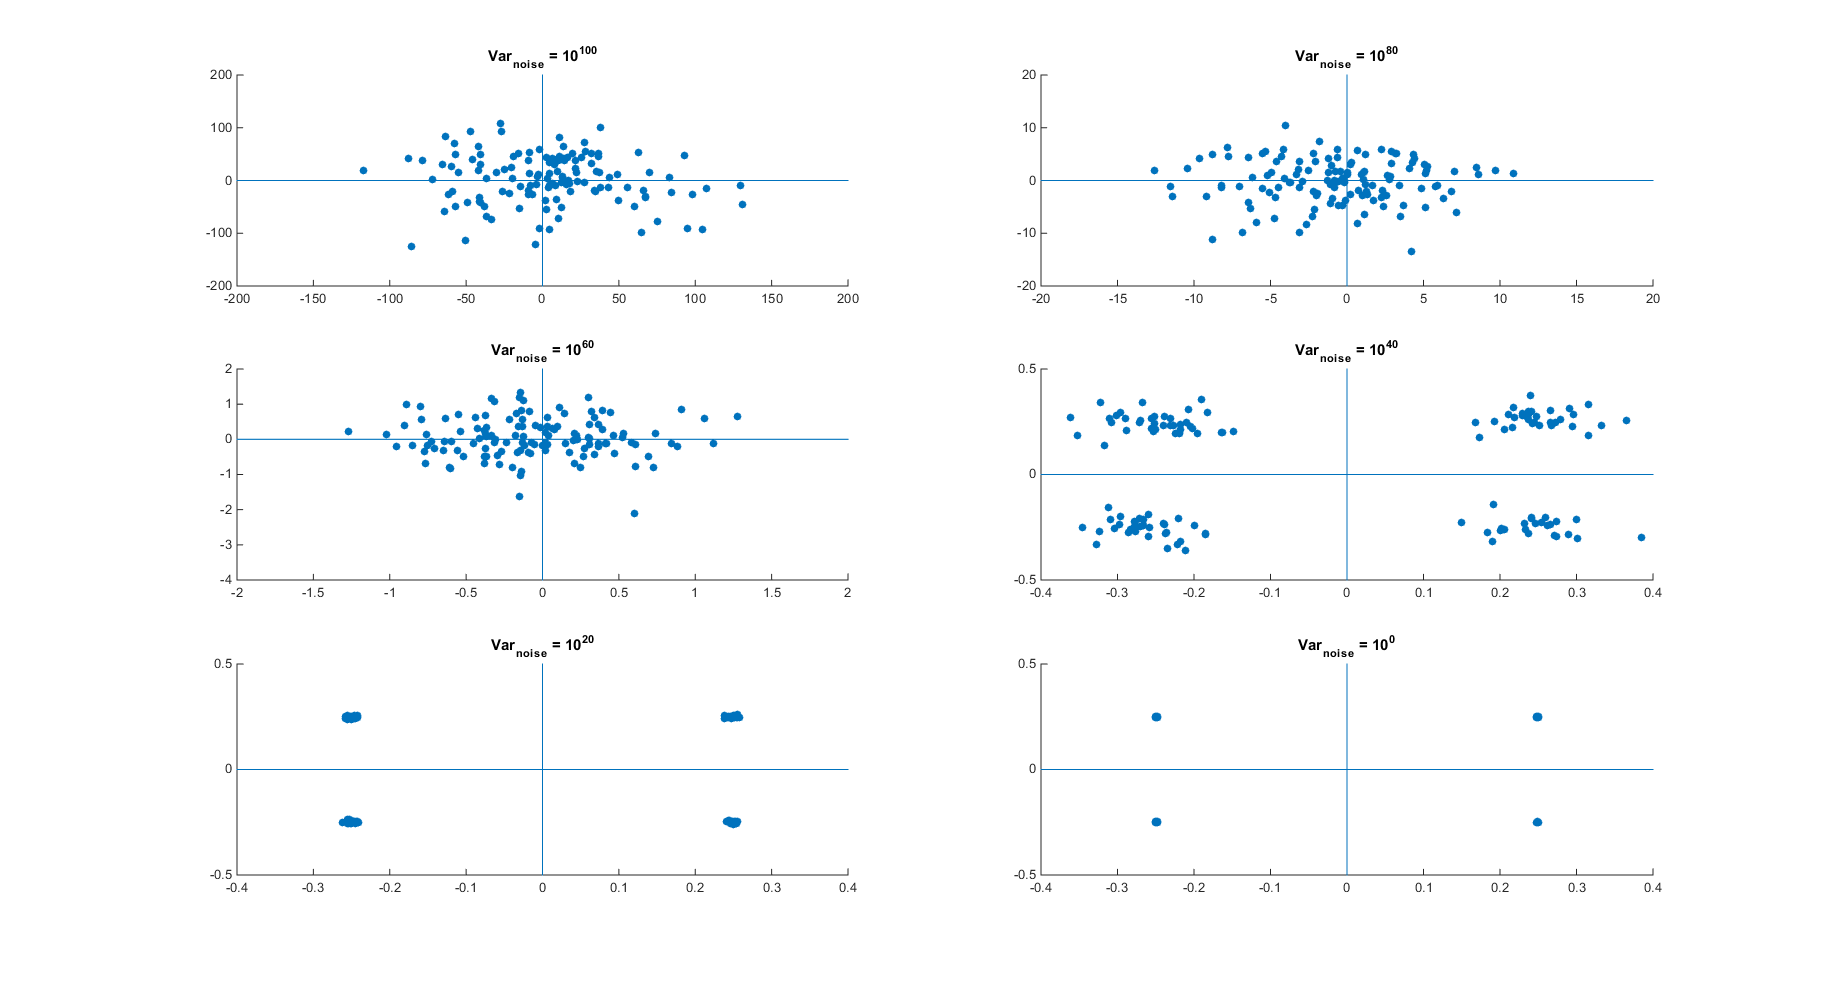
\includegraphics[width=6.625in, height=4in]{../3.Transferring0and1/Q2PC.png}}
\caption{توزیع خطا در فضای 2 بعدی به ازای دنباله 128 بیتی}
\label{fig}
\end{figure}
همانطور که دیده می شود با افزایش واریانس نویز ابر دور نقاط صحیح پیوسته بزرگتر می شود، در توان $10^{40}$ هنوز خطا قابل قبول است اما همانطور که دیده می شود در گام بعدی ابر ها کاملا با هم قاطی شده اند و دیگر نمی توان بیت ها را به صورت درست بازیابی کرد.
\\
\subsection{مقایسه دو روش تشکیل پالس}
با مقایسه هیستوگرام 2 بعدی این دو شکل پالس (به خصوص در توان $10^{40}$) در می یابیم از آن جایی که ابر احتمالی مربوط به این شکل موج بزرگتر است نویز تاثیر بیشتری روی تخریب کیفیت انتقال داده داشته است، پس انتخاب ما استفاده از نوع پالس اولی است، البته موضوع مهم دیگری که هست این است که کانال اطلاعاتی که به صورت فیلتر میان گذر است، سیگنال تک فرکانسی مانند این نوع پالس را کمتر آسیب می زند.
\clearpage

\section{انتقال دنباله ای از اعداد 8 بیتی}
کد های مربوط به توابع این قسمت در $./Functions$ و کد های مربوط به مشخصات سیستمی در $./4.8bitTransferring$ آمده است.
\subsection{SourceGenerator and OutputDecoder}
کد این قسمت در $./Functions/SourceGenerator.m$ آمده است و در آن به سادگی اعداد ورودی توسط تابع $de2bi$ به عدد های مبنای 2 تبدیل می شوند، اما کارکرد عجیب این تابع به شکلی است که اعداد را به صورت برعکس خروجی می دهد (از آن جایی که در سمت گیرنده میخواهیم از معکوس همین تابع استفاده کنیم مشکلی پیش نمی آید، ولی از نظر اصولی به نظر می رسد بهتر است این مورد درست شود)، بدین ترتیب ستون های این ماتریس را برعکس میکنیم و سپس ترانهاده این ماتریس را به فرم برداری در می آوریم که آماده ارسال باشد.
\\
تابع بعدی که در $./Functions/OutputDecoder.m$ آمده است دقیقا کار برعکس را انجام می دهد ابتدا بردار را به یک ماتریس چند در 8 تبدیل میکند و پس از قرینه کردن ستون ها آن را به تابع $bi2de$ می دهد و خروجی را به شکل برداری تحویل خروجی می دهد.
\\
\subsection{Byte Transferring}
کد های مربوط به این قسمت در $./4.8bitTransferring$ آمده است.
\\
مشخصات سیستم دقیقا مشابه قسمت قبلی است تنها تفاوتی که در این قسمت وجود دارد آن است که ورودی ها ابتدا به شکل اعداد 8 بیتی داده میشوند (که تفاوتی برای سیتم ندارد و تنها حجم ورودی آن بیشتر میشود)، در واقع فرق مهم تر این قسمت را قسمت قبل این است که برخلاف قسمت قبل که خطا تنها به صورت تبدیل 0 به 1 یا برعکس دیده می شد اینجا به صورت تغییر یک عدد از بازه $(0,255)$ به بازه $(0,255)$ منتقل می شود و می توانیم از رابطه زیر واریانس آماری آنان را محاسبه کنیم:
$$
\Sigma^{N}_{n=1} (b - \hat{b})^2
$$
حاصل این عبارت می تواند عدد بزرگی باشد زیرا تغییر کوچکی در بیت پر ارزش یک عدد می تواند خطای بسیار زیادی تولید بکند، به همین دلیل تصویر مربوط به واریانس خطا بر حسب واریانس نویز اختشاش زیادی دارد زیرا یکی از همین تغییرات غیر منتظره می تواند به کلی روند را عوض بکند:
\begin{figure}[htbp]
\centerline{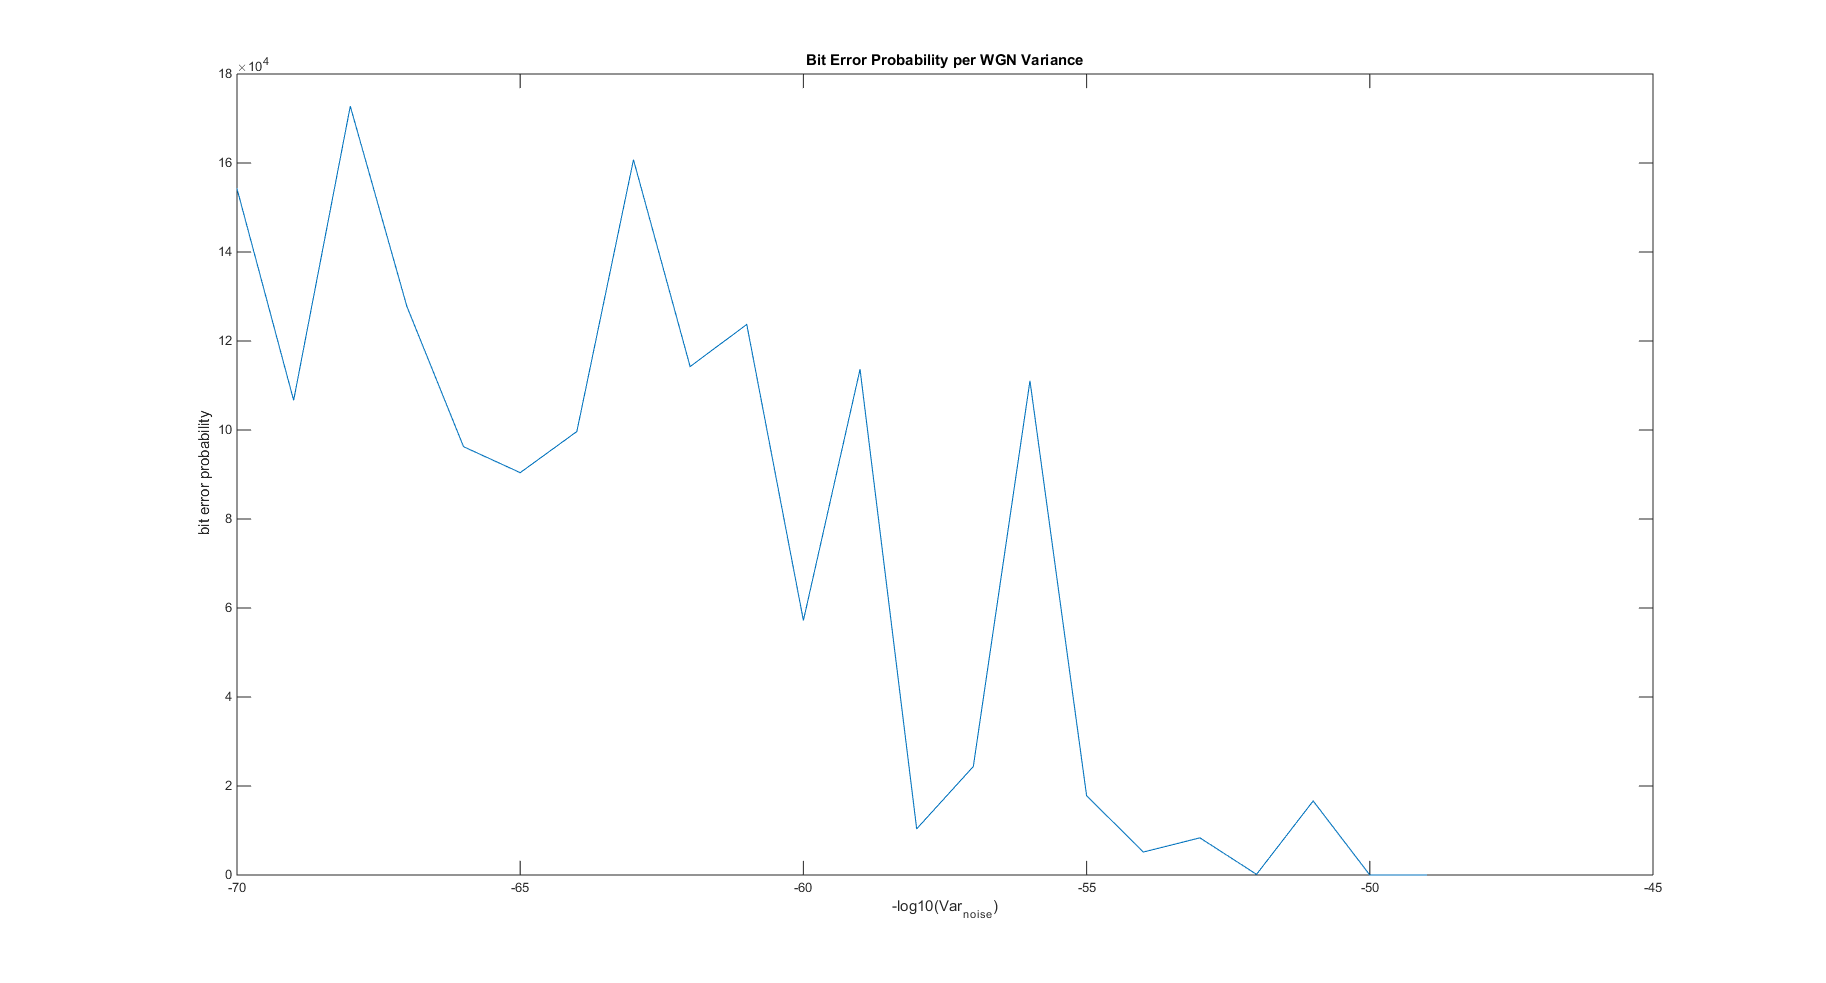
\includegraphics[width=6.625in, height=4in]{../4.8bitTransferring/Q2_16Byte.png}}
\caption{واریانس خطا بر حسب واریانس نویز به ازای دنباله 16 بایتی}
\label{fig}
\end{figure}
\subsection{Error Histogram}
در این قسمت متغییر تصادفی زیر را تعریف میکنیم، هدف آن است که تخمین بزنیم این توزیع با افزایش تعداد نمونه ها و توان نویز به چه توزیعی همگرا خواهد شد:
$$
X = B - \hat{B}
$$
\\
برای این قسمت واریانس نویز های زیر را امتحان میکنیم:
$$
\sigma^2 = \{10^{100}, 10^{60}, 10^{40}, 1\}
$$
و برای نشان دادن توزیع احتمالی که باید در ازای افزایش نویز به آن همگرا شویم از $hist$ با 50 بازه بندی استفاده میکنیم و خواهیم داشت:
\begin{figure}[htbp]
\centerline{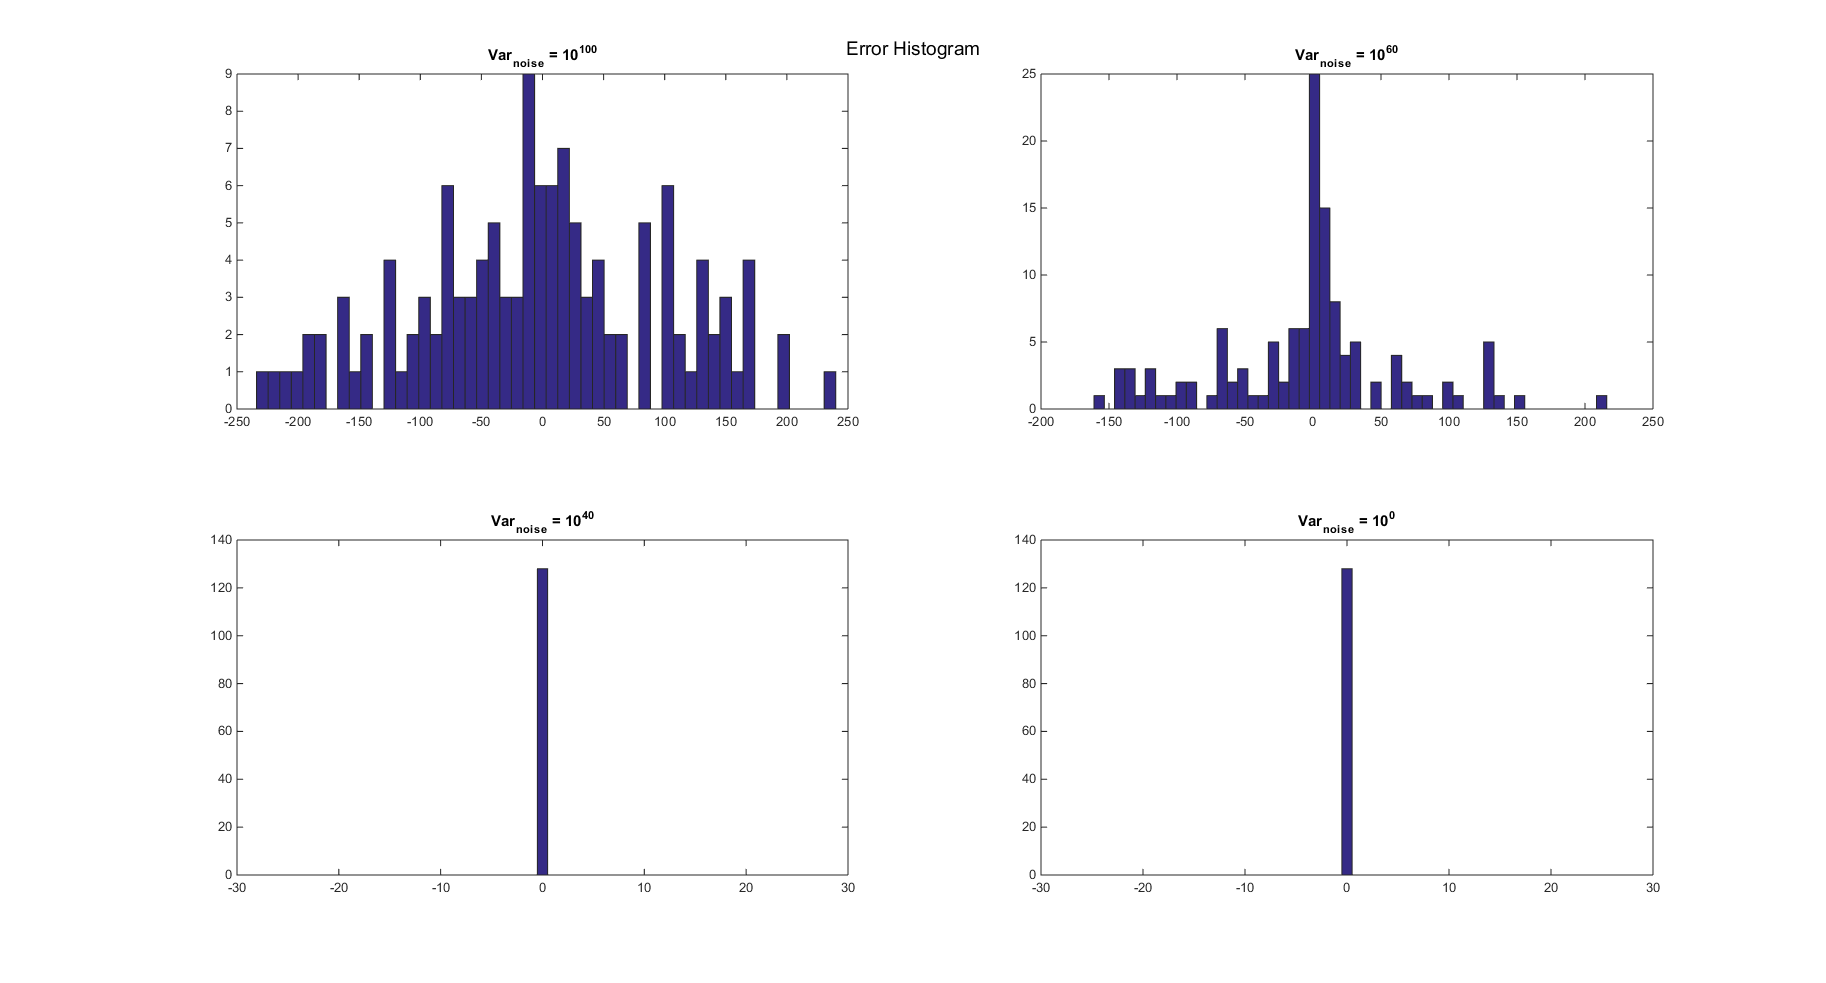
\includegraphics[width=6.625in, height=4in]{../4.8bitTransferring/Q3_128Byte.png}}
\caption{هسیتوگرام تجربی توزیع حطا در ازای افزایش واریسانس نویز با دنباله 128 بایتی}
\label{fig}
\end{figure}
همانطور که دیده می شود، در نویزهای کوچک توزیع احتمالی متمرکز روی صفر است و خطا وجود ندارد، برای حدس زدن توزیع متغییر تصادفی $X$ کافی است در حالتی که نویز بینهایت می شود میتوان فرض کرد که ارتباط بین $B$ و $\hat{B}$ از بین می رود و گویی از یکدیگر مستقل می شوند، بدین ترتیب هر دوی آن ها توزیع $U(0,255)$ دارند، نیز می توان گفت $\hat{B}-$ نیز توزیع یکنواحت به فرم  $U(-255,0)$ است و از آنجایی که می دانیم توزیع احتمالاتی یک متغییر تصادفی که جمع 2 متغییر تصادفی دیگر است به صورت کانولوشن توزیع آن دو جمع شونده آنان است، با کانوالو کردن این دو توزیع احتمالا در همدیگر یک توزیع احتمالی مثلثی در بازه $(-255, 255)$ به وجود می آید که برای تابع چگالی احتمال بودن می بایست انتگرال 1 داشته باشد و در نتیجه ماکسیموم آن برابر خواهد بود با $\frac{1}{255}$.
\\
میتوان تابع زیر را برای چگالی احتمال این توزیع در نظر گرفت:
$$
f_X(x)=\left\{
    \begin{array}{ll}
         \frac{1}{255} - \frac{|y|}{255^2} & |y| < 255 \\
        0 & \mbox{o.w.}
    \end{array}
\right.
$$
\subsection{Var(Error)}
با توجه به تحلیل بدست آمده در قسمت قبل داریم($E[X] = 0 $) :
$$
Var(X) = E[(X - E[X])^2] = E[X^2] = \int_{-\infty}^{\infty} x^2 \times f_X(x) dx 
$$
$$
= \int_{-255}^{255} x^2 \times (\frac{1}{255} - \frac{|y|}{255^2}) dx = 2\int_{0}^{255} x^2 \times (\frac{1}{255} - \frac{y}{255^2}) dx
$$
$$
2(\frac{255^2}{3} - \frac{255^2}{4}) = \frac{255^2}{6}
$$
$$
\sigma = \frac{255}{\sqrt[2]{6}} = 104.103
$$
که تقریبا برابر با 104 است که میتوان از هسیتوگرام تجربی نیز چنین حسی پیدا کرد.
\clearpage
\section{کدینگ منبع}
\subsection{Some Codings}
\subparagraph{آ)}
مشکلی کدینگ $C_1 $ این است که کد $10$ مربوط به دو سمبل $b$ و $d$ است. این موضوع باعث می شود که در هنگام بازیابی ندانیم که باید به جای این کد، کدام یک از سمبل ها را جاگذاریم کنیم.
\\
\subparagraph{ب)}
مشکلی کدینگ $C_2 $ این است که کد $010$ هم میتواند کد مربوط به $d$ باشد و هم کد دو سمبل کنار هم قرار گرفته شده $ab$ باشد، در نتیجه باز هم نمیتوان رابطه یکتایی بین کدینگ و سمبل ایجاد کرد.
\\
\subparagraph{ج)}
مشکلی کدینگ $C_2 $ این است که با دریافت $0$ نمیدانیم که آیا این کد مروبط به حرف $a$ است و یا ابتدا کد مروبط به سمبل های دیگر است، با دریافت بقیه اعداد نیز همین اتفاق می افتد، زیرا همه ی کدینگ های زیر رشته کدینگ بعد خود هستند و تا زمانی که یک $0$ دیگر نیاید متوجه نمی شویم که آیا مخابره این سمبل تمام شده است یا خیر.
\subsection{New Coding}
همانطور که گفته شد میخواهیم مسئله بهینه سازی زیر را به روش لاگرانژ حل کنیم:
$$
min \Sigma^M_{i=1} p_il_i
$$
$$
when:\Sigma^M_{i=1} 2^{-l_i} = 1
$$
پس تابع انرژی لاگرانژ را به شکل زیر تشکیل می دهیم:
$$
L(\lambda, l_1, ..., l_M) = E[l(X)] - \lambda(1 - \Sigma^M_{i=1} 2^{-l_i}) = p_1l_1 + ... + p_1l_M  - \lambda(1 - 2^{-l_1} -...- 2^{-l_M})
$$
حال شروط ضرایب لاگرانژ را اعمال می کنیم:
$$
\frac{\partial L}{\partial \lambda} = 0 \rightarrow 1 = \Sigma^M_{i=1} 2^{-l_i}
$$
که شرطی است که ما می خواستیم، و:
$$
\forall i \in [1,M] : \frac{\partial L}{\partial l_i} = 0 \rightarrow p_i - \lambda ln(2) 2^{-l_i} = 0
$$
که می دهد:
$$
l_i = log_2(\frac{\lambda ln(2)}{p_i})
$$
و از طرفی از قانون احتمال کل می دانیم:
$$
\Sigma^M_{i=1} p_i = \Sigma^M_{i=1} \lambda ln(2) 2^{-l_i} = \lambda ln(2) \Sigma^M_{i=1} 2^{-l_i} = 1 
$$
$$
\lambda = \frac{1}{ln(2)}
$$
که خواهیم داشت:
$$
l_i = log_2(\frac{1}{p_i}) = -log_2(p_i)
$$
\\
\subsection{Applications}
در جدول زیر قدم به قدم این کار را انجام می دهیم:
\begin{center}
  \begin{tabular}{ c | c | c | c | c | c | c}
    \hline
    i & 1 & 2 & 3 & 4 & 5 & 6 \\ \hline
    $symbol$ & a & b & c & d & e & f \\ \hline
    $p_i$ & $\frac{1}{2}$ & $\frac{1}{4}$ & $\frac{1}{8}$ & $\frac{1}{16}$ & $\frac{1}{32}$ & $\frac{1}{32}$ \\ \hline
    $l_i = -log_2(p_i)$ & 1 & 2 & 3 & 4 & 5 & 5 \\ \hline
    $code$ & 0 & 10 & 110 & 1110 & 11110 & 11111
  \end{tabular}
\end{center}
بدین صورت سمبلی که احتمال رخ دادنش کمتر است طول کد بیشتر و سمبلی با احتمال رخ داد زیاد طول کد بیشتری دارد.
\\
\subsection{E[l(X)]}
داریم:
$$
E[l(X)] = p_1l_1 + p_2l_2 + p_3l_3 + p_4l_4 + p_5l_5 + p_6l_6
$$
$$
= \frac{1}{2}\times 1 + \frac{1}{4}\times 2 + \frac{1}{8}\times 3 + \frac{1}{16}\times 4 + \frac{1}{32}\times 5 + \frac{1}{32}\times 5
$$
$$
= 1.9375
$$
\\
\subsection{InformationSource}
کد ها مربوط به این قسمت در $./5.SourceCoding/InformationSource$ قرار دارد.
\\
در این تابع با دریافت عدد $n$ یک بردارد به همین اندازه از اعداد رندوم تولید می کنیم که اعداد بین $(0,31)$ را به صورت یکنواخت تولید میکند. در گام بعدی یک سری ماسک می سازیم که هرکدام بازه ای از اعداد را مشغول میکند که طول این بازه متناسب با احتمال آنان در $X$ است. در گام بعدی حاصلضرب این ماسک ها در مقادیر متناظرشان با هم جمع می شود و خروجی به تابع $char$ داده می شود و این تابع فرم رشته ای آن را به عنوان خروجی بر می گرداند.
\\
\subsection{SourceEncoder}
کد ها مربوط به این قسمت در $./5.SourceCoding/SourceEncoder$ قرار دارد.
\\
در این تابع با یک حلقه روی کارکتر های رشته ورودی تصمیم میگیریم که چه رشته ای از 0 و 1 ها را به بردار خروجی اضافه کنیم، ساختاری کاملا ساده و قابل حدس، تنها نکته آنجاست که اندیس بردار خروجی باید هر مرحله به تعداد  $l_i$ جلو برود
\\
\subsection{SourceDecoder}
کد ها مربوط به این قسمت در $./5.SourceCoding/SourceDecoder$ قرار دارد.
\\
در این تابع نیز با توجه به ویژگی خوب پیشوندی بودن کدینگ روی خانه های ورودی حرکت میکنیم و با دیدن صفر، یک $a$ به رشته خروجی اضافه میکنیم، در غیر این صورت (یعنی اولین بیت  1 است) اگر بیت دوم 0 بود فورا $b$ اضافه می کنیم و همین روند را ادامه می دهیم تا به پایان رشته برسیم، در هر مرحله $l_i$ اندیس حرکت کننده روی دنباله ورودی را جلو می بریم.

یکی از مشکلات احتمالی زمانی است که نویز این کدینگ را تحت تاثیر قرار دهد، در آن صورت این روش، روش خوبی برای بازیابی نیست.
\\
\subsection{$H_n(X)$}
کد مربوط به این قسمت در $./5.SourceCoding/Q8 $ قرار دارد.
\\
یک بردار از مقادیر مختلف $n$ می سازیم و در داخل یک حلقه به ازای هر $n$ ابتدا یک دنباله از حروف $X$ به طول $n$ می سازیم و سپس از آن یک دنباله بیتی می سازیم، بعد از این کار دوباره توسط تابع بازیابی آن را بازیابی می کنیم.
\\
در پایان هر دور نسبت اندازه کل دنباله بیت ها (مجموع طول رشته ها) را بر تعداد حروف تقسیم میکنیم (معیاری از میانگین)، از آن جایی که این داده ها هم توزیع هستند و $I.I.D$ طبق قانون همگرایی میانگین آماری به امید ریاضی (تخمین امید ریاضی) این عدد می بایست در اعداد بزرگ همگرا به مقدار امید ریاضی طول کدینگ باشد، و همانطور که می بینید، این موضوع در شکل زیر نشان داده شده است:
\begin{figure}[htbp]
\centerline{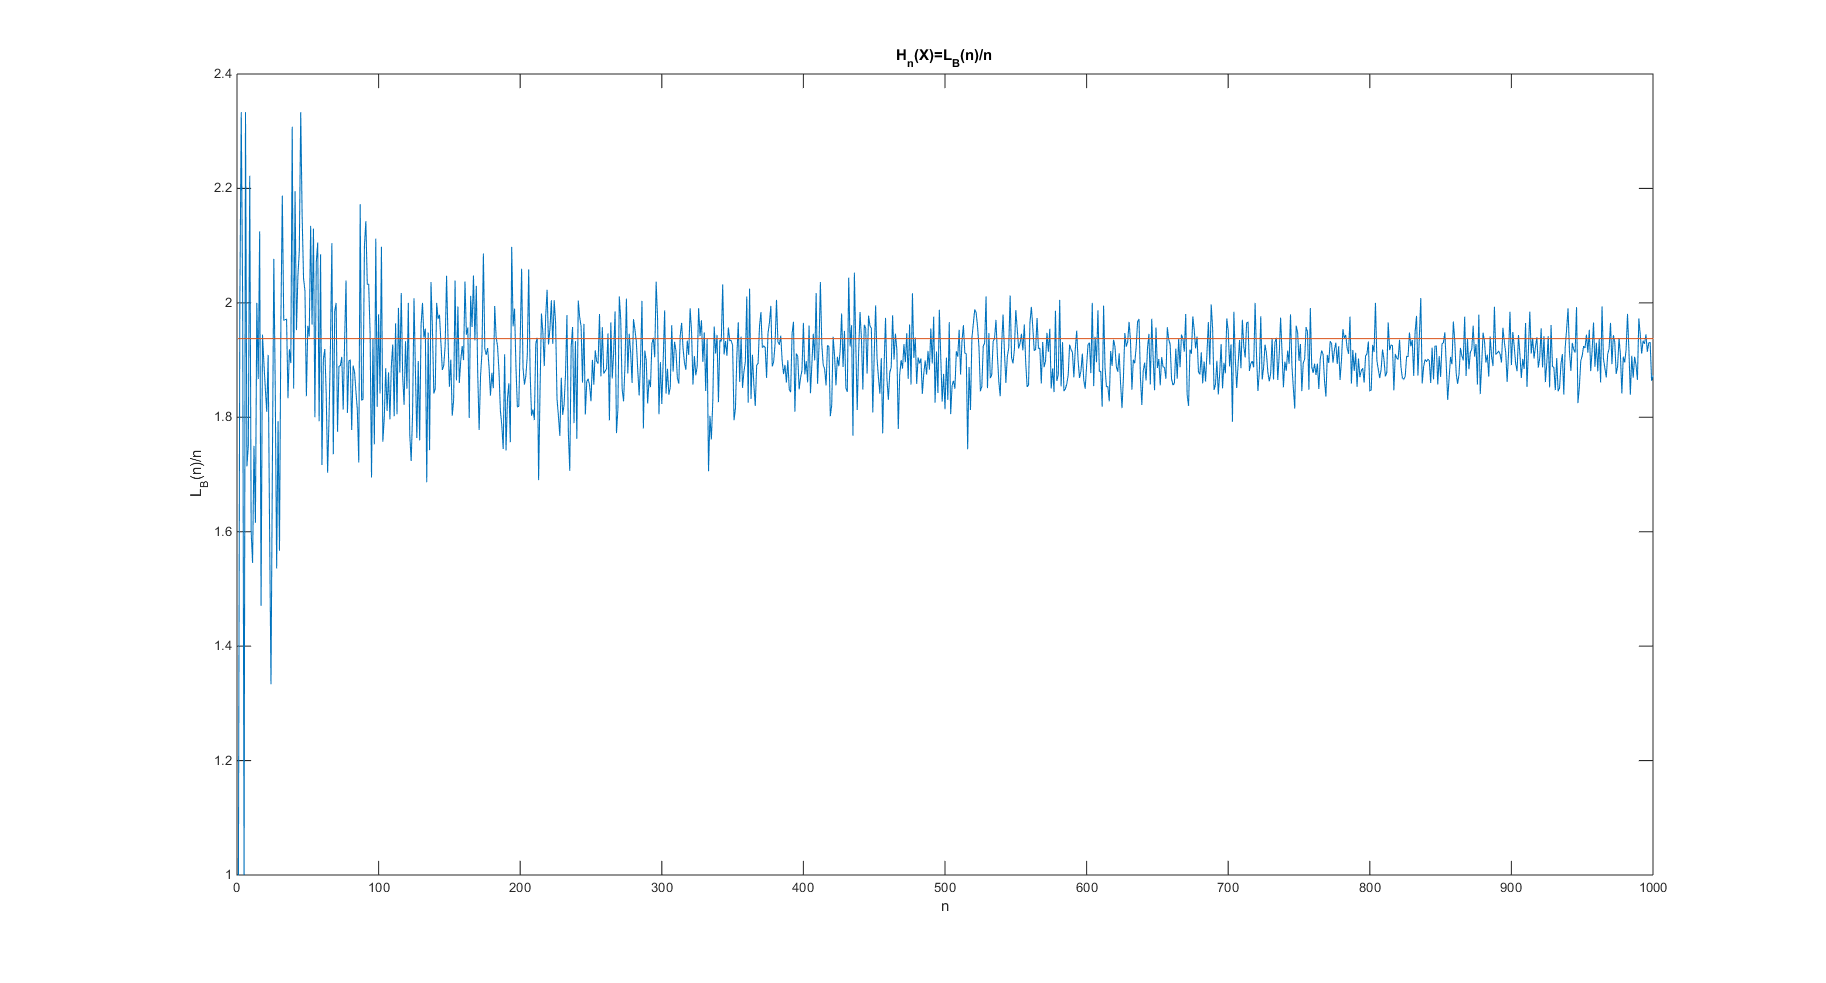
\includegraphics[width=6.625in, height=4in]{../5.SourceCoding/Q8.png}}
\caption{همگرایی میانگین تجربی به امید ریاضی با افزایش تعداد دادگان}
\label{fig}
\end{figure}
\\
\subsection{Distortion}
با توجه به راهنمایی، بازه بودن $A,B$ و از طرفی لزوم تعریف شدن دامنه تعریف در تمام اعداد حقیقی، نقطه ای مانند $c$ وجود دارد که مرز بین این دو ناحیه است (بدون کاهش از کلیت فرض میکنیم $B = (-\infty, c)$ و $A = (c, \infty)$، پس خواهیم داشت:
$$
D = E[(X-\hat{X})^2] = \int_{-\infty}^{\infty} \int_{-\infty}^{\infty} (x-\hat{x})^2 d\hat{x}f_{X,\hat{X}}(x,\hat{x})dx
$$
$$
= \int_{-\infty}^{c} \int_{-\infty}^{\infty} (x-\hat{x})^2 d\hat{x}f_{X,\hat{X}}(x,\hat{x})dx + \int_{c}^{\infty} \int_{-\infty}^{\infty} (x-\hat{x})^2 d\hat{x}f_{X,\hat{X}}(x,\hat{x})dx
$$
با توجه به تعریف، در انتگرال اول، متغییر $\hat{X}$ می بایست برابر $\hat{x_2}$ و در انتگرال دوم برابر $\hat{x_1}$ است:
$$
= \int_{-\infty}^{c} (x-\hat{x_2})^2 f_X(x) dx + \int_{c}^{\infty}(x-\hat{x_1})^2 f_X(x) dx
$$
$$
= \int_{-\infty}^{c} (x^2 - 2x\hat{x_2}+\hat{x_2}^2) f_X(x)dx + \int_{c}^{\infty}(x^2 -2x\hat{x_1} +\hat{x_1}^2) f_X(x) dx
$$
$$
= \int_{-\infty}^{\infty} x^2 f_X(x) dx - 2(\hat{x_2} \int_{-\infty}^{c} x f_X(x) dx + \hat{x_1} \int_{c}^{\infty} x f_X(x) dx) +  \hat{x_2}^2 \int_{-\infty}^{c} f_X(x) dx + \hat{x_1}^2 \int_{c}^{\infty} f_X(x) dx
$$
و نیز میدانیم:
$$
\int_{-\infty}^{c} x f_X(x) dx + \int_{c}^{\infty} x f_X(x) dx = \int_{-\infty}^{\infty} x f_X(x) dx = E[X] = 0 
$$
$$
\int_{-\infty}^{c} f_X(x) dx + \int_{c}^{\infty} f_X(x) dx = \int_{-\infty}^{\infty} f_X(x) dx = 1
$$
پس با جایگذاری داریم:
$$
D = \sigma^2 -2(\hat{x_2} - \hat{x_1}) \int_{-\infty}^{c} x f_X(x) dx + (\hat{x_2}^2 - \hat{x_1}^2) \int_{-\infty}^{c} f_X(x) dx
$$
برای رسیدن به نقطه مینیموم:
$$
\frac{\partial D}{\partial c} = 0 \rightarrow -2(\hat{x_2} - \hat{x_1})cf_X(c) +  (\hat{x_2}^2 - \hat{x_1}^2) f_X(c) = 0
$$
$$
*:(\hat{x_2} - \hat{x_1})(\hat{x_2} + \hat{x_1} - 2c) = 0
$$
$$
\frac{\partial D}{\partial \hat{x_1}} = 0 \rightarrow 2(1 -\hat{x_1})\int_{-\infty}^{c} x f_X(x) dx = 0 \rightarrow \hat{x_1} = 1
$$
$$
\frac{\partial D}{\partial \hat{x_2}} = 0 \rightarrow 2(1 +\hat{x_2})\int_{-\infty}^{c} x f_X(x) dx = 0 \rightarrow \hat{x_2} = -1 
$$
$$
* \rightarrow c = \frac{\hat{x_2} + \hat{x_1}}{2} = 0
$$
$$
p(\hat{X} = \hat{x_1})=P(\hat{X} = \hat{x_1}) = P(X \in A) = P(X \in A) =  0.5 \int_{-\infty}^{\infty} f_X(x) dx = 0.5
$$
\end{document}